\chapter{A Greedy Optimal Point-to-Point Content Routing Schema for DTN}
\label{chapter:ptp}
\minitoc

Mobile ad hoc networks (MANETs) had been treated, until recently, as a connected graph over which
end-to-end paths need to be established. This legacy view might no longer be appropriate for modelling existing and emerging wireless networks~\cite{Fall:DTNrouting,Fall:Sigcomm05,Glance:pollen}. Wireless propagation phenomena, node mobility, power management, etc. often result in intermittent connectivity with end-to-end paths either lacking or rapidly changing. To allow some services to operate even under these challenging conditions, researchers have proposed a new networking paradigm, often referred to as Delay Tolerant Networking (DTN~\cite{dtnrg}), based on the \emph{store-carry-and-forward} routing principle~\cite{Fall:DTNrouting}. Nodes there, rather than dropping a session when no forwarding opportunity is available, store and carry messages until new communication opportunities arise.

Despite a large amount of effort invested in the design of efficient routing algorithms for DTNs, there has not been a similar focus on queue management and message scheduling. Yet, the combination of long-term storage and the, often expensive, message replication performed by many DTN routing protocols~\cite{Vahdat:epidemic,Lindgren:probabilistic} impose a high bandwidth and storage overhead on wireless
nodes~\cite{akis:ton-multi}. Moreover, the data units disseminated in this context, called \emph{bundles}, are self-contained, application-level data units, which can often be large~\cite{dtnrg}. As a result, it is expected that nodes' buffers, in this context, will often operate at full capacity. Similarly, the available bandwidth during a contact could be insufficient to communicate all intended messages. Consequently, \emph{regardless of the specific routing algorithm used}, it is important to have: \emph{(i)} efficient drop policies to decide which message(s) should be discarded when a node's buffer is full, and \emph{(ii)} efficient scheduling policies to decide which message(s) should be chosen to exchange with another encountered node when bandwidth is limited and in which order.

In this chapter, we solve this problem in its foundation. We develop a theoretical framework based on Epidemic message dissemination~\cite{haas:mobihoc03,Inria:MessageDelay,akis:mobihoc06}, and propose an optimal joint scheduling and drop policy, GBSD (Global knowledge Based Scheduling and Drop) that can maximize the average delivery rate or minimize the average delivery delay. GBSD derives a per-message utility by taking into account all information that are relevant for message delivery, and manages messages accordingly. Yet, to derive these utilities, it requires \textit{global} network information, making its implementation difficult in practice, especially given the intermittently connected nature of the targeted networks. In order to amend this, we propose a second policy, HBSD (History Based Scheduling and Drop), a distributed (\textit{local}) algorithm based on statistical learning. HBSD uses network history to estimate the current state of required (\textit{global}) network parameters and uses these estimates, rather than actual values (as in GBSD), to calculate message utilities for each performance target metric.

To our best knowledge, the recently proposed RAPID protocol~\cite{Levine:Sigcomm07} is the only effort aiming at scheduling (and to a lesser extend message drop) using a similar theoretical framework. Yet, the utilities derived there are sub-optimal, as we will explain later, and require global knowledge (as in GBSD), raising the same implementation concerns. Simulations using both synthetic mobility models and real traces show that our HSBD policy not only outperforms existing buffer management and scheduling policies (including RAPID), but can also approximate the performance of the reference GBSD policy, in all considered scenarios.

Furthermore, we look deeper into our distributed statistics collection solution and attempt to identify the available tradeoffs between the collection overhead and the resulting performance. Aggressively collecting statistics and exchanging them with every encountered node allows estimates to converge faster, but it can potentially result in high energy and bandwidth consumption, and also interfere with data transmissions. Our results suggest that close to optimal performance can still be achieved even when the signaling overhead is forced (through sampling) to take only a small percentage of the contact bandwidth.

Finally, we examine how our algorithm behaves under different congestion regimes. Interestingly, we find that \emph{(i)} at low to moderately congested regimes, the optimal policy is simply equivalent to dropping the message with the oldest age (similarly to the findings of \cite{QueuingPolicies}), while \emph{(ii)} at highly congested regimes, the optimal policy is not linear on message age; some young messages have to be dropped, as a means of indirect admission control, to allow older messages to create enough replicas and have a chance to be delivered. Hence, our framework can also explain what popular heuristic policies are doing, in this context, relative to the optimal one.

The rest of this chapter is organized as follows. Section~\ref{sec:optimal-policy} describe the ''reference'', optimal joint scheduling and drop policy that uses global knowledge about the network. Then, we present in Section~\ref{sec:learning} a learning process that enables us to approximate the global network state required by the reference policy. Section~\ref{sec:sims} discusses our evaluation setup and presents performance results for both policies (GBSD and HBSD) using synthetic and real mobility traces. In Section~\ref{sec:NetworkHistory}, we examine in detail our mechanism to collect and maintain network history statistics, and evaluate the signaling-performance tradeoff. Section~\ref{sec:HBSDUtilitiesDistributions} studies the behavior of our HBSD policy in different congestion regimes. Finally, we conclude this chapter and present some future investigation directions in Section~\ref{sec:conclusion}.

\section{Optimal Joint Scheduling and Drop Policy}
\label{sec:optimal-policy}

In this section, we first describe our problem setting and the assumptions for our theoretical framework. We then use this framework to identify the optimal policy, GBSD (Global Knowledge based Scheduling and Drop). This policy uses global knowledge about the state of each message in the network (number of replicas). Hence, it is difficult to implement it in a real world scenario, and will only serve as reference. In the next section, we will propose a distributed algorithm that can successfully approximate the performance of the optimal policy.

\subsection{Assumptions and Problem Description}
\label{subsec:ProblemDescription}

We assume there are $L$ total nodes in the network. Each of these nodes has a buffer, in which it can store up to $B$ messages in transit, either messages belonging to other nodes or messages generated by itself. Each message has a Time-To-Live ($TTL$) value, after which the message is no more useful to the application and should be dropped by its source and all intermediate nodes. The message can also be dropped when a notification of delivery is received, or if an ''anti-packet'' mechanism is implemented~\cite{Towsley:Epidemic}.

\textbf{Routing:} Each message has a single destination (unicast) and is assumed to be routed using a replication-based scheme~\cite{akis:ton-multi}. During a contact, the routing scheme used will create a list of messages to be replicated among the ones currently in the buffer. Thus, different routing schemes might choose different messages. For example, epidemic routing will replicate all messages not already present in the encountered node's buffer~\cite{Vahdat:epidemic}. For the purposes of this work, we will use epidemic routing as a case study, for the following reasons. First, its simplicity allows us to concentrate on the problem of resource allocation, which is the focus of this work. Second, it consumes the most resources per message compared to any other scheme. As a result, it can be easily driven to medium or high congestion regimes, where the efficient resource allocation problem is most critical. Third, given the nature of random forwarding schemes, unless a buffer is found full or contact capacity is not enough to transfer all messages, epidemic forwarding is optimal in terms of delay and delivery probability. Consequently, epidemic routing along with appropriate scheduling and message drop policies, can be viewed as a new routing scheme that optimally adapts to available resources~\cite{Levine:Sigcomm07}. Finally, we note that our framework could be used to treat other types of traffic (e.g. multicast), as well. However, we focus on unicast traffic to elucidate the basic ideas behind our approach, and defer the treatment of multi-point traffic to future work.

\textbf{Mobility Model:} Another important element in our analytical framework is the impact of mobility. In the DTN context, message transmissions occur only when nodes encounter each other. Thus, \emph{the time elapsed between node meetings is the basic delay component}. The meeting time distribution is a basic property of the mobility model assumed~\cite{akis:mobihoc06,Inria:MessageDelay}. By \emph{meeting time} we refer to the time until two nodes starting from the stationary distribution come within range (''first meeting-time''). If some of the nodes in the network are static, then one needs to use \emph{hitting times} between mobile and static nodes. Our theory can be easily modified to account for static nodes by considering, for example, two classes of nodes with different meeting rates (see e.g.~\cite{akis09}). To formulate the optimal policy problem, we will first assume a class of mobility models that has the following properties:
\begin{enumerate}
\item [A.1] Meeting times are exponentially distributed or have at least an \emph{exponential tail};
\item [A.2] Nodes move \emph{independently} of each other;
\item [A.3] Mobility is homogeneous, that is, all node pairs have the same meeting rate $\lambda$.
\end{enumerate}

Regarding, the first assumption, it has been shown that many simple synthetic mobility models like Random Walk, Random Waypoint and Random Direction~\cite{akis:mobihoc06,Inria:MessageDelay} have such a property. Furthermore, it is a known result in the theory of random walks on graphs that hitting times on subsets of vertices usually have an exponential tail~\cite{Aldous:book}. Finally, it has recently been argued that meeting and inter-meeting times observed in many traces also exhibit an exponential tail~\cite{LeBoudec:Mobicom07}. As we will see in Section~\ref{subsec:MaxAvgDeliveryRate}, in our framework, \emph{we sample the remaining meeting time only when a drop or scheduling decision needs to be taken}. In a sparse network (as in our case), it can be shown that, at this time, the two nodes in question have already \emph{mixed} with high probability. Thus, the quantity sampled can be approximated by the meeting time from stationarity, or the tail of the inter-meeting time distribution, which, as explained, is often exponential~\cite{Akis:IJAACS2008}. In other words, it is not required to make the stronger assumption of Poisson distributed inter-meeting times, as often done in related literature.

Regarding the second assumption, although it might not always hold in some scenarios, it turns out to be a useful approximation. In fact, one could use a mean-field analysis argument to show that independence is not required, in the limit of large number of nodes, for the analytical formulas derived to hold (see e.g.~\cite{LeBoudec:Sigmetrics09}).

Finally, in Section~\ref{section:heterogeneous-mobility}, we discuss how to remove assumption [A.3] and generalize our framework to heterogenous mobility models.

\textbf{Buffer Management and Scheduling:} Let us consider a time instant when a new contact occurs between nodes $i$ and $j$. The following resource allocation problem arises when nodes are confronted with limited resources (i.e. contact bandwidth and buffer space). We note that, by ''limited resources'', we do not imply that our focus is only small, resource-limited nodes (e.g. wireless sensors), but rather that the offered forwarding or storage load exceeds the available capacity. In other words, we are interested in congestion regimes.

(\emph{Scheduling Problem}) If $i$ has $X$ messages in its \emph{local} buffer that it should forward to $j$ (chosen by the routing algorithm), but does not know if the contact will last long enough to forward all messages, which ones should it send first, so as to maximize the \emph{global} delivery probability for \emph{all} messages currently in the network?

(\emph{Buffer Management Problem}) If one (or more) of these messages arrive at $j$'s buffer and find it full, what is the best message $j$ should drop among the ones already in its buffer (\emph{locally}) and the newly arrived one, in order to maximize, let's say, the average delivery rate among all messages in the network (\emph{globally})?

To address these two questions, we propose the following policy. Given a routing metric to optimize, \emph{our policy, GBSD, derives a per-message utility that captures the \emph{marginal value} of a given message copy, with respect to the chosen optimization metric}. Based on this utility, two main functions are performed:

\begin{enumerate}
\item \emph{Scheduling}: at each contact, a node should replicate messages in decreasing order of their utilities.
\item \emph{Drop}: when a new message arrives at a node with a full buffer, this node should drop the message with the smallest utility among the one just received and the buffered messages.
\end{enumerate}

\begin{figure}[!h]
\centering
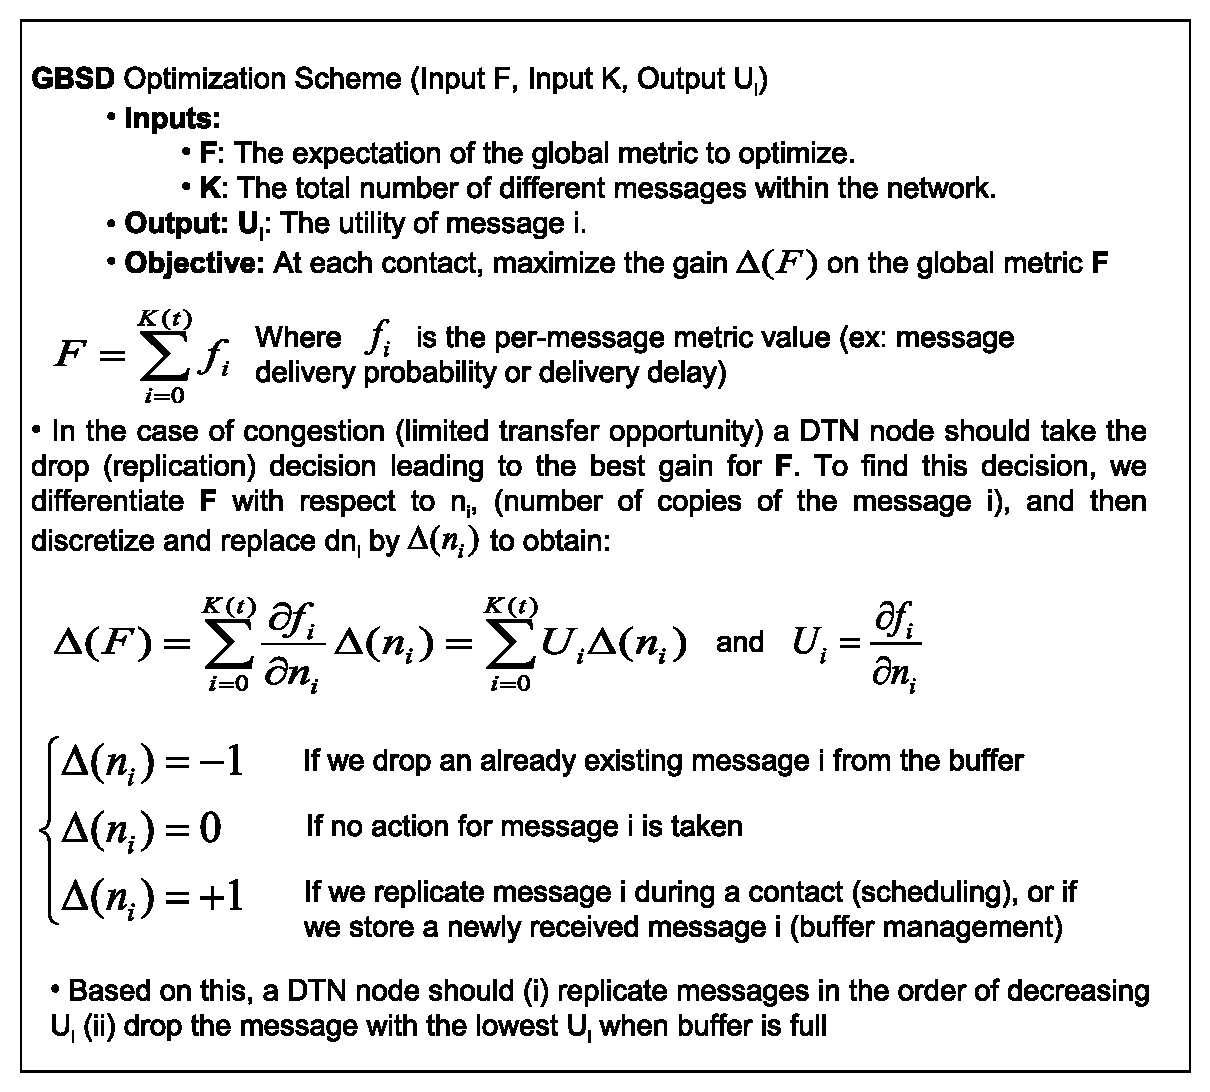
\includegraphics[width=3.1in,height=3in]{Chapitre3/GOS.eps}
\caption{GBSD Global optimization policy}
\label{GlobalOptimizationSchema}
\end{figure}

We will derive next such a per-message utility for two popular metrics: maximizing the average delivery probability (rate), and minimizing the average delivery delay. Table~\ref{table:notation} contains some useful notation that we will use throughout this chapter. Finally, the GBSD optimization policy is summarized in Figure~\ref{GlobalOptimizationSchema}.

\begin{table}
\caption{Notation}
\centering
\label{table:notation}
\footnotesize
\begin{tabular}{|p{1.8cm}|p{5.7cm}|}
\hline
\bfseries Variable & \bfseries Description\\
\hline
L & Number of nodes in the network\\
\hline
K(t) & Number of distinct messages in the network at time $t$\\
\hline
$TTL_i$ & Initial Time To Live for message $i$\\
\hline
$R_i$ & Remaining Time To Live for message $i$\\
\hline
$T_i$ = $TTL_i$ - $R_i$ & Elapsed Time for message $i$. It measures the time since this message was generated by its source\\
\hline
$n_i(T_i)$ & Number of copies of message $i$ in the network after elapsed time $T_i$\\
\hline $m_i(T_i)$ & Number of nodes (excluding source) that
have \emph{seen} message $i$ since its creation until elapsed time $T_i$\\
\hline
$\lambda$ & Meeting \emph{rate} between two nodes; $\lambda = \frac{1}{E[H]}$ where $E[H]$ is the average meeting time\\
\hline
\end{tabular}
\end{table}
\normalsize

\subsection{Maximizing the average delivery rate}
\label{subsec:MaxAvgDeliveryRate}
We first look into a scenario where each message has a \emph{finite} $TTL$ value. The source of the message keeps a copy of it during the whole $TTL$ duration, while intermediate nodes are not obliged to do so. To maximize the average delivery probability among all messages in the network, the optimal policy must use the per message utility derived in the following theorem, in order to perform scheduling and buffer management.

\begin{theorem}\label{th:delivery-rate}
Let us assume that there are $K$ messages in the network, with
elapsed time $T_{i}$ for the message $i$. For each message $i \in [1,K]$, let $n_i(T_i)$ be the number of nodes who have a copy of the message at this time instant, and $m_i(T_i)$ those that have ``seen'' the message (excluding the source) since its creation ($n_i(T_i) \leqslant m_i(T_i)+1)$. We say that a node \emph{A} has ''seen'' a message $i$, when $A$ had received a copy of message $i$ in the past, regardless of whether it still has the copy or has already removed it from its buffer. To maximize the average delivery rate of all messages, a DTN node should apply the GBSD policy using the following utility per message $i$:

\begin{equation}\label{eq:GBSD-delivery-rate}
U_{i}(DR) = (1-\frac{m_i(T_i)}{L-1})\lambda R_i\exp(-\lambda n_i(T_i) R_i).
\end{equation}
\end{theorem}

The probability that a copy of a message $i$ will not be delivered by a node is given by the probability that the next meeting time with the destination is greater than $R_i$, the remaining lifetime of a message ($R_{i} = TTL - T_{i}$). This is equal to $\exp(-\lambda{R_i})$ under our assumptions.

Knowing that message $i$ has $n_i(T_i)$ copies in the network, and assuming that the message has not yet been delivered, we can derive the probability that the message itself will not be delivered (i.e. none of the $n_{i}$ copies gets delivered):

\begin{eqnarray}
P\{\mbox{message\ $i$ not\ delivered}\ |\ \mbox{not\ delivered\ yet}  \}= \nonumber \\
\prod_{k=1}^{n_i(T_i)}\exp(-\lambda R_i ) = \exp(-\lambda n_i(T_i) R_i).
\label{eq:p-not-delivered}
\end{eqnarray}

We need to also take into consideration what has happened in the network since the message generation, in the absence of an explicit delivery notification (this part is not considered in RAPID~\cite{Levine:Sigcomm07}, making the utility function derived there suboptimal). Given that all nodes including the destination have the same chance to see the message, the probability that a message $i$ has been already delivered is equal to:

\begin{align}
P \{ \mbox{message\ $i$ already\ delivered} \} &=& m_i(T_i) / (L-1).
\label{eq:p-already-delivered}
\end{align}

Combining Eq.(\ref{eq:p-not-delivered}) and Eq.(\ref{eq:p-already-delivered}), the probability that a message $i$ will get delivered before its $TTL$ expires is:

\vspace{-0.4cm}
\small
\begin{align*}
P_i & =  P \{ \mbox{message\ $i$ not\ delivered\ yet} \} *  (1 -\exp(-\lambda n_i(T_i) R_i)) \\
& +  P \{ \mbox{message\ $i$ already delivered} \} \\
& =  (1 - \frac{m_i(T_i)}{L-1})*(1 - \exp(-\lambda n_i(T_i) R_i ))+\frac{m_i(T_i)}{L-1}.
\end{align*}
\normalsize

So, if we take at instant $t$ a snapshot of the network, the global delivery rate for the whole network will be:

\vspace{-0.4cm}
\small
\begin{align*} DR =\sum_{i=1}^{K(t)}\left[(1 - \frac{m_i(T_i)}{L-1})*(1 -\exp(-\lambda n_i(T_i)  R_i )) +\frac{m_i(T_i)}{L-1}\right].
\end{align*}
\normalsize

In case of a full buffer or limited transfer opportunity, a DTN node should take respectively a drop or replication decision that leads to the best gain in the global delivery rate DR. To define this optimal decision, we differentiate DR with respect to $n_i(T_i)$,

\small
\begin{align*}
\Delta(DR) &= \sum_{i=1}^{K(t)}{\frac{\partial P_i}{\partial n_i(T_i)} * \bigtriangleup n_i(T_i)}
\\&= \sum_{i=1}^{K(t)} \left[{(1-\frac{m_i(T_i)}{L-1})\lambda R_i\exp(-\lambda n_i(T_i) R_i) * \bigtriangleup n_i(T_i)}\right]
\end{align*}
\normalsize

Our aim is to maximize $\Delta(DR)$. In the case of message drop, for example, we know that: $\Delta n_i(T_i) = -1$ if we drop an already existing message $i$ from the buffer, $\Delta n_i(T_i) = 0$ if we don't drop an already existing message $i$ from the buffer, and $\Delta n_i(T_i) = +1$ if we keep and store the newly-received message $i$. Based on this, GBSD ranks messages using the per message utility in Eq.(\ref{eq:GBSD-delivery-rate}), then schedules and drops them accordingly. This utility can be viewed as the \emph{marginal utility value} for a copy of a message $i$ with respect to the total delivery rate. The value of this utility is a function of the global state of the message $i$ ($n_i$ and $m_i$) in the network.

As is evident from the above description, the GBSD policy is a greedy, locally optimal policy. However, greedy policies in general, are not guaranteed to converge to globally optimal outcomes. We will investigate the optimality properties of GBSD further in Section~\ref{OptimalityOfGradientPolicy}.

\subsection{Minimizing the average delivery delay}
\label{subsec:MinAvgDeliveryDelay}

We next turn our attention to minimizing the average delivery delay. We now assume that all messages generated have infinite $TTL$ or at least a $TTL$ value large enough to ensure a delivery probability close to $1$. The following Theorem derives the optimal per-message utility, for the same setting and assumptions as Theorem~\ref{th:delivery-rate}.

\begin{theorem} \label{th:delivery-delay}
To minimize the average delivery delay of all messages, a DTN node should apply the GBSD policy using the following utility for each message $i$:

\begin{equation}\label{eq:delivery-delay}
U_{i}(DD) = \frac{1}{n_i(T_i)^2 \lambda} ( 1-\frac{m_i(T_i)}{L-1}). \end{equation}
\end{theorem}

Let us denote the delivery delay for message $i$ with random variable $X_i$. This delay is set to $0$ (or any other constant value) if the message has been already delivered. Then, the total expected delivery delay ($DD$) for all messages for which copies still exist in the network is given by,

\small
\begin{align}\label{eq:DD1}
DD & = \sum_{i=1}^{K(t)} \left[\frac{m_i(T_i)}{L-1}*0 + (1 - \frac{m_i(T_i)}{L-1}) * E[X_i | X_i
> T_i]\right].
\end{align}
\normalsize

We know that the time until the first copy of the message $i$ reaches the destination follows an exponential distribution with mean $1/(n_i(T_i)\lambda)$. It follows that,

\begin{align}\label{eq:DD2}
E[X_i | X_i
> T_i] &= T_i + \frac{1}{n_i(T_i) \lambda}.
\end{align}

Substituting Eq.(\ref{eq:DD2}) in Eq.(\ref{eq:DD1}), we get,

\begin{align*}
DD &= \sum_{i=1}^{K(t)} (1 - \frac{m_i(T_i)}{L-1})(T_i + \frac{1}{n_i(T_i)
\lambda}).
\end{align*}

Now, we differentiate $D$ with respect to $n_i(T_i)$ to find the policy that maximizes the improvement in $D$,

\begin{align*}
\Delta(DD) &= \sum_{i=1}^{K(t)}{\frac{1}{n_i(T_i)^2 \lambda} ( \frac{m_i(T_i)}{L-1}-1)* \Delta n_i(T_i)}.
\end{align*}

The best drop or forwarding decision will be the one that maximizes $\vert\Delta(DD)\vert$ (or $-\Delta(DD)$). This leads to the per message utility in Eq.(\ref{eq:delivery-delay}).


Note that, the per-message utility with respect to delivery delay is different than the one for the delivery rate. This implies (naturally) that both metrics cannot be optimized concurrently.

\subsection{The Case of Non-Homogeneous Mobility}
\label{section:heterogeneous-mobility}

Throughout our analysis, we have so far assumed homogeneous node mobility. Recent measurement studies have revealed that, often, different node pairs might have different meeting rates. We extend here our analytical framework, in order to derive per-message utilities that maximize the global performance metric, in face of such heterogeneous mobility scenarios. We illustrate the extension with the delivery rate. The treatment of delivery delay utilities does not involve Laplace transforms, but poses no extra difficulties. Specifically, we assume that meetings between a given node pair are exponentially distributed with meeting rate $\tilde{\lambda}$, where $\tilde{\lambda}$ is a \emph{random variable} such that:

\begin{equation*}
\tilde{\lambda} \in [0,\infty), \mbox{distributed as } f(\tilde{\lambda}).
\end{equation*}

$f(\tilde{\lambda})$ is a probability distribution that models the heterogeneous meeting rates between nodes, and can be any function integrable in $[0,\infty)$, capturing thus a very large range of conceivable mobility models.

The analysis of Theorem~\ref{th:delivery-delay} is thus modified as follows. Let's assume that message $i$ has $n_{i}$ copies in the network, and that the $n_{i}$ carriers have (unknown) meeting rates $\tilde{\lambda_{1}},\tilde{\lambda_{2}},\dots,\tilde{\lambda_{n_{i}}}$, respectively. Eq.(\ref{eq:p-not-delivered}) becomes:

\begin{eqnarray}
P\{\mbox{message\ $i$ not\ delivered}\ |\ \mbox{not\ delivered\ yet}  \}= \nonumber \\
E_{\tilde{\lambda_{1}},\tilde{\lambda_{2}},\dots,\tilde{\lambda_{n_{i}}}} [ \prod_{j=1}^{n_i}\exp(-\tilde{\lambda_{j}} R_i ) ] = \\
\prod_{j=1}^{n_i} \int_{0}^{\infty} \exp(-\tilde{\lambda_{j}} R_i ) f(\tilde{\lambda_{j}}) d\lambda_{j}  = (F_{\mathcal{L}}(R_{i}))^{n_{i}}, \label{eq:conditional-delivery}
\end{eqnarray}

where $F_{\mathcal{L}}(R_{i})$ is the Laplace transform of distribution $f(x)$ evaluated at $R_{i}$. Continuing as in the proof of Theorem~\ref{th:delivery-delay}, we get the unconditional probability of delivery $P_{i}$:

\begin{equation*}
P_{i} = (1 - \frac{m_i}{L-1})* (F_{\mathcal{L}}(R_{i}))^{n_{i}}+\frac{m_i}{L-1}.
\end{equation*}

Differentiating $P_{i}$ with respect to $n_{i}$, we derive the following generic marginal utility per message:

\begin{equation} \label{eq:general-utility-delivery}
(1 - \frac{m_i}{L-1}) * \ln(F_{\mathcal{L}}(R_{i})) * (F_{\mathcal{L}}(R_{i}))^{n_{i}}.
\end{equation}

We now consider some example distributions for node meeting rates, and derive the respective marginal utility.

\emph{Dirac delta funtion}: Let $f(\tilde{\lambda}) = \delta(\tilde{\lambda} - \lambda)$, where $\delta(x)$ is an impulse function (Dirac's delta function). This corresponds to the case of homogeneous mobility, considered earlier, with average meeting rates for all nodes equal to $\lambda$. The laplace distribution of $f(\tilde{\lambda})$ is then equal to $F_{\mathcal{L}}(R_{i}) = \exp(-\lambda R_{i})$. Replacing this in Eq.(\ref{eq:general-utility-delivery}), the generic marginal utility, gives us Eq.(\ref{eq:GBSD-delivery-rate}), the utility for homogeneous mobility, as expected.

\emph{Exponential distribution}: Let $f(\tilde{\lambda}) = \lambda_{0} \exp(-\tilde{\lambda} \lambda_{0})$, for $\tilde{\lambda} \ge 0$. This corresponds to a mobility model, where individual rates between pairs differ, but the variance of these rates is not high and their average is equal to $\lambda_0$. The laplace transform of $f(\tilde{\lambda})$ is

\begin{equation*}
F_{\mathcal{L}}(R_{i}) = \frac{1}{(R_{i} + \lambda_{0})^{2}}.
\end{equation*}
Replacing this in Eq.(\ref{eq:general-utility-delivery}) gives us the marginal utility per message that should be used:
\begin{equation}
(1 - \frac{m_i}{L-1}) * \ln(\frac{1}{(R_{i} + \lambda_{0})^{2}}) * \frac{1}{(R_{i} + \lambda_{0})^{2n_{i}}}.
\end{equation}

\emph{Unknown distribution in large networks}: If the actual probability distribution of meeting rates is not known, the following approximation could be made in order to derive marginal utilities per message and use them for buffer management. Let us assume that the meeting rates come from an unknown distribution with first and second moments $\bar{\lambda}$ and $\sigma^{2}$, respectively. Let us further assume that there is a large number of nodes, such that $n_{i}$, the number of copies of message $i$ at steady state, is large. Using the central limit theorem, we have:

\begin{equation}
Prob(\sum_{j=1}^{n_{i}} \tilde{\lambda_{j}} \le \lambda) \underset{n_{i} \rightarrow \infty}{\sim} \mathcal{N}(n_{i}\bar{\lambda}, \sigma \sqrt{n_{i}}),
\end{equation}

that is, the sum of meeting rates with the destination of the $n_{i}$ relays for message $i$ is (approximately) normally distributed. Replacing this in Eq.(\ref{eq:conditional-delivery}), we get the (unconditional) delivery probability $P_{i}$

\begin{eqnarray*}
P_{i} = (1 - \frac{m_i}{L-1})* F_{\mathcal{L}}(R_{i}) + \frac{m_i}{L-1},
\end{eqnarray*}

where $F_{\mathcal{L}}(R_{i})$ is the Laplace transform of the above normal distribution. Note that the Laplace transform is not raised anymore to the $n_{i}^{\mbox{th}}$ power, as the distribution already corresponds to the sum of all rates. After some algebraic manipulations we can get the new marginal utility for message $i$:

\footnotesize
\begin{equation}
(1 - \frac{m_i}{L-1}) * \frac{ (\bar{\lambda}^{2} \sqrt{8} (n_{i})^{-\frac{1}{2}} + \sqrt{2} \sigma^{2} (n_{i})^{-\frac{5}{2}}) \exp( n_{i} \frac{\bar{\lambda}^{2}}{\sigma^{2}} + \frac{R_{i}^{2}}{4} )}{8 \sigma^{4}} * \mbox{erfc}(\frac{R_{i}}{2}).
\end{equation}
\normalsize

In a large enough network, even if the actual distribution of meeting rates is not known, a node could still derive good utility approximations, by measuring and maintaining an estimate for the first and second moments of observed or reported meeting rates (e.g. with techniques similar to the ones discussed in the next Section). Furthermore, the homogeneous assumption could be considered as a useful approximation for large networks where the common rate is taken as $\bar{\lambda}$. Additional complexity in the mobility model (e.g. correlated meeting rates) could still be handled in our framework, yet at the expense of ease of interpretation (and thus usefulness) of the respective utilities. We will therefore consider the simple case of homogeneous mobility for the remainder of our discussion, in order to better elucidate some additional key issues related to buffer management in DTNs, and resort to a simulation-based validation under realistic mobility patterns.

\subsection{Optimality of Gradient Ascent Policy}
\label{OptimalityOfGradientPolicy}

We finally turn our attention back to the distributed (\emph{local}) buffer management policies of Sections~\ref{subsec:MaxAvgDeliveryRate} and~\ref{subsec:MinAvgDeliveryDelay}, in order to further investigate their optimality. Let us observe our network at a random time instant, and assume there are $K$ total undelivered messages, with remaining Times To Live $R_{1}, R_{2}, \dots, R_{K}$, respectively. The centralized version of our buffer management problem then consists of assigning the available buffer space across the network ($L$ nodes each able to store $B$ message copies) among the copies of these messages, $n_{1}, n_{2}, \dots, n_{K}$, so as to maximize the expected delivery probability for all these messages (where the expectation is taken over mobility decisions of all nodes). This corresponds to the following optimization problem:

\begin{eqnarray}
\underset{n_{1},n_{2},\dots,n_{K}}{\max} \sum_{i=1}^{K} (1-\exp(-\lambda n_i R_i)) \label{eq:optimization-function} \\
\sum_{i=1}^{K} n_{i} - L B \le 0 \label{eq:capacity-constraint} \\
n_{i} - L  \le 0, \forall i \label{eq:max-copy-constraint} \\
n_{i} \geq 1, \forall i \label{eq:min-copy-constraint}
\end{eqnarray}

This is a constrained optimization problem, with $K$ variables and $2K+1$ inequality constraints. The optimization function in Eq.(\ref{eq:optimization-function}) is a concave function in $n_{i}$. Constraint in Eq.(\ref{eq:capacity-constraint}) says that the total number of copies (for all messages) should not exceed the available buffer space in all $L$ nodes, and is linear. Finally, the $2K$ constraints of Eq.(\ref{eq:max-copy-constraint}) are also linear, and simply say that there is no point for any node to store two copies of the same message. Consequently, if we assume that $n_{i}$ are real random variables (rather than integers), this is a \emph{convex optimization} problem, which can be solved efficiently~\cite{Boyd:convex-optimization-book} (but not easily analytically).

Having found an optimal vector $\mathbf{n}$, a centralized optimal algorithm can easily assign the copies to different nodes (e.g. picking nodes sequentially and filling their buffers up with any non-duplicate copy, starting from the messages with highest assigned $n_{i}$ --- due to uniform mobility the choice of specific nodes does not matter). It is important to note that, given this assignment, \emph{no further message replication or drop is needed. This is the optimal resource allocation averaged over all possible future node movements.} The optimal algorithm must perform the same process at every subsequent time step in order to account for new messages, messages delivered, and the smaller remaining times of undelivered messages.

Our local policies offer a \emph{distributed implementation of a gradient ascent algorithm for this problem}. Gradient ascent algorithms look at the current state, i.e. vector $\mathbf{n}(k)$ at step $k$, and choose a neighboring vector $\mathbf{n}(k+1)$ that improves the optimization function in Eq.(\ref{eq:optimization-function}), and provably converge to the optimal solution~\cite{Boyd:convex-optimization-book}. In our case, a step corresponds to a \emph{contact} between two nodes, and the neighboring states and permitted transitions depend on the messages in the buffers of the two nodes in contact. In other words, our gradient ascent algorithm is supposed to make enough steps to converge to the optimal copy vector $\mathbf{n^{*}}$, before the state of the network (i.e. number and ID of messages) changes enough for the optimal assignment to change significantly. This depends on the rate of update steps ($\approx \lambda L^{2}$) and the message TTL. If $TTL * \lambda * L^{2} \gg 1$, then we expect the distributed, local policy to be able to closely follow the optimal solution at any time $t$. In Section~\ref{GBSD:Optimality}, we use simulation to prove that this is indeed the case for the scenarios considered.

\section{Using Network History to Approximate Global Knowledge in Practice}
\label{sec:learning}

It is clear from the above description that the optimal policy (GBSD) requires global information about the network and the ''spread'' of messages, in order to optimize a specific routing metric. In particular, for each message present in a node's buffer, we need to know the values of $m_i(T_i)$ and $n_i(T_i)$. In related work~\cite{Levine:Sigcomm07}, it has been suggested that this global view could be obtained through a secondary, ``instantaneous'' channel (e.g. cellular network), if available, or by flooding (``in-band'') all necessary meta-data. Regarding the former option, cellular network connections are known to be low bandwidth (measurements suggest only few kbps even for 2.5-3G technologies~\cite{Keshav:multi-nic}) and high cost in terms of power and actual monetary cost per bit. In networks of more than a few nodes, the amount of signalling data might make this option prohibitive. Concerning flooding, our experiments show that the impact of the flooding delay on the performance of the algorithm is not negligible. In practice, intermittent network connectivity and the long time it takes to flood buffer status information across DTN nodes, make this approach inefficient.

A different, more robust approach is to find estimators for the unknown quantities involved in the calculation of message utilities, namely $m$ and $n$. We do this by designing and implementing a learning process that permits a DTN node to gather knowledge about the global network state at different times in the past, by making in-band exchanges with other nodes. Each node maintains a list of encountered nodes and the state of each message carried by them as a function of time (i.e. its buffer state history). Specifically, it logs whether a given message was present at a given time $T$ in a node's buffer (counting towards $n$) or whether it was encountered earlier but is not anymore stored, e.g. it was dropped (counting towards $m$). In Section~\ref{sec:NetworkHistory}, we describe our statistics maintenance and collection method, in more detail, along with various optimizations to considerably reduce the signalling overhead.

Since global information gathered thus about a specific message might take a long time to propagate (as mentioned earlier) and hence might be obsolete when we calculate the utility of the message, we follow a different route. Rather than looking for the current value of $m_{i}(T)$ and $n_{i}(T)$ \emph{for a specific message $i$} at an elapsed time $T$, we look at what happens, \emph{on average, for all messages after an elapsed time $T$}. In other words, the $m_i(T)$ and $n_i(T)$ values for message $i$ at elapsed time $T$ are estimated using measurements of $m$ and $n$ for the same elapsed time $T$ but \emph{measured for (and averaged over) all other older messages}. These estimations are then used in the evaluation of the per-message utility.

Let's denote by $\stackrel{\wedge}{n}(T)$ and $\stackrel{\wedge}{m}(T)$ the estimators for $n_i(T)$ and $m_i(T)$ of message $i$. For the purpose of the analysis, we suppose that the variables $m_{i}(T)$ and $n_{i}(T)$ at elapsed time $T$ are instances of the random variables $N(T)$ and $M(T)$. We develop our estimators $\stackrel{\wedge}{n}(T)$ and $\stackrel{\wedge}{m}(T)$ so that when plugged into the GBSD's delivery rate and delay per-message utilities calculated in Section~\ref{sec:optimal-policy}, we get two new per-message utilities that can be used by a DTN node without any need for global information about messages. This results in a new scheduling and drop policy, called HBSD (History Based Scheduling and Drop), a deployable variant of GBSD that uses the same algorithm, yet with per-message utility values calculated using estimates of $m$ and $n$.

\subsection{Estimators for the Delivery Rate Utility}
\label{sec:learning:EDR}

When global information is unavailable, one can calculate the average delivery rate of a message over all possible values of
$M(T)$ and $N(T)$, and then try to maximize it. In the framework of the GBSD policy, this is equivalent to choosing the estimators $\stackrel{\wedge}{n}(T)$ and $\stackrel{\wedge}{m}(T)$ so that the calculation of the average delivery rate is unbiased:

\begin{align*}
E[(1 - \frac{M(T)}{L-1})*(1 -\exp(-\lambda N(T) R_i
))+\frac{M(T)}{L-1}]&=
\\(1 -
\frac{\stackrel{\wedge}{m}(T)}{L-1})*(1 -\exp(-\lambda
\stackrel{\wedge}{n}(T) R_i
))+\frac{\stackrel{\wedge}{m}(T)}{L-1}
\end{align*}

Plugging any values for $\stackrel{\wedge}{n}(T)$ and $\stackrel{\wedge}{m}(T)$ that verify this equality into the expression for the per-message utility of Eq.(~\ref{eq:GBSD-delivery-rate}), one can make sure that the obtained policy maximizes the average delivery rate. This is exactly our purpose. Suppose now that the best estimator for $\stackrel{\wedge}{m}(T)$ is its average, i.e., $\stackrel{\wedge}{m}(T)=\stackrel{-}{m}(T)=E[M(T)]$. This approximation is driven by the observation we made that the histogram of the random variable $M(T)$ can be  approximated by a Gaussian distribution with good accuracy. To confirm this, we have applied the Lillie test~\cite{LillieTest}, a robust version of the well known Kolmogorov-Smirnov goodness-of-fit test, to $M(T)$ for different elapsed times ($T$ = 25\%,50\% and 75\% of the $TTL$). This test led to acceptance for a 5\% significance level. Consequently, the average of $M(T)$ is at the same time the unbiased estimator and the most frequent value among the vector $M(T)$. Then, solving for $\stackrel{\wedge}{n}(T)$ gives:

\begin{align}
\stackrel{\wedge}{n}(T) = -\frac{1}{\lambda R_i}
\ln(\frac{E[(1-\frac{M(T)}{L-1})\exp(-\lambda N(T)
R_i)]}{(1-\frac{\stackrel{-}{m}(T)}{L-1})})
\end{align}

Substituting this expression into Eq.(\ref{eq:GBSD-delivery-rate}) we obtain the following new per message utility for our approximating HBSD policy:

\begin{align}
\label{HBSD-DR-U}
\lambda R_i E[(1-\frac{M(T)}{L-1})\exp( - \lambda R_i N(T))]
\end{align}

The expectation in this expression is calculated by summing over all known values of $N(T)$ and $M(T)$ for past messages at elapsed time $T$. Unlike Eq.(\ref{eq:GBSD-delivery-rate}), this new per-message utility is a function of past history of messages and can be calculated locally. It maximizes the average message delivery rate calculated over a large number of messages. When the number of messages is large enough for the law of large numbers to work, our history based policy should give the same result as that of using the real global network information.

Finally, we note that $L$, the number of nodes in the network, could also be calculated from the statistics maintained by each node in the network. In this work, we assume it to be fixed and known, but one could estimate it similar to $n$ and $m$, or using different estimation algorithms like the ones proposed in~\cite{PellegriniAOC2009}.

\subsection{Estimators for the Delivery Delay Utility}
\label{sec:learning:EDD}

Similar to the case of delivery rate, we calculate the estimators $\stackrel{\wedge}{n}(T)$ and $\stackrel{\wedge}{m}(T)$ in such a way that the average delay is not affected by the estimation. This gives the following per-message utility specific to HBSD,

\begin{align}
\label{HBSD-DD-U}
\frac{E[\frac{L-1-M(T)}{N(T)}]^2}{\lambda
(L-1)(L-1-\stackrel{-}{m}(T))}
\end{align}

This new per-message utility is only a function of the locally available history of old messages and is thus
independent of the actual global network state. For large number of messages, it should lead to the same average delay
as when the exact values for $m$ and $n$ are used.


\section{Performance Evaluation}
\label{sec:sims}

\subsection{Experimental Setup}
\label{sec:ExperimentalSetup}

To evaluate our policies, we have implemented a DTN framework into the Network Simulator NS-2~\cite{DTN-NS2}. This implementation includes \emph{(i)} the Epidemic routing protocol with \emph{FIFO} for scheduling messages queued during a contact and \emph{drop-tail} for message drop, \emph{(ii)} the RAPID routing protocol based on flooding (i.e. no side-channel) as described, to our best
understanding, in~\cite{Levine:Sigcomm07}, \emph{(iii)} a new version of Epidemic routing enhanced with our optimal joint scheduling and drop policy (GBSD), \emph{(iv)} another version using our statistical learning based distributed algorithm (HBSD), and \emph{(v)} the VACCINE anti-packet mechanism described in~\cite{Towsley:Epidemic}. Note that we have also performed simulations without any anti-packet mechanism, from which similar conclusions can be drawn.

In our simulations, each node uses the 802.11b protocol to communicate, with rate 11Mbits/sec. The transmission range is 100 meters, to obtain network scenarios that are neither fully connected (e.g. MANET) nor extremely sparse. Our simulations are based on five mobility scenarios: two synthetic mobility models and three real-world mobility traces.

\emph{Synthetic Mobility Models:} We've considered both the Random Waypoint mobility model and the HCMM model~\cite{HCMM}. HCMM is a mobility model inspired by Watts' Caveman model that was shown to reproduce statistics of human mobility, such as inter-contact times and contact duration. In HCMM, the Caveman model is used to define a graph (overlay) with nodes divided into (well connected) groups and each group is assigned to a physical home location. Also, some users belonging to different groups can have links to each other (bridges). These (intra- and inter-group) links are used in HCMM to drive movements: each user moves towards a given group's home location with a probability proportional to the weight of its links towards the group.

\emph{Real Mobility Traces:} The first \emph{(i)} real trace is the one collected as part of the ZebraNet wildlife tracking experiment in Kenya and described in~\cite{ZebraNetMovement}. The second mobility trace tracks San Francisco's Yellow Cab taxis. Many cab companies outfit their cabs with \emph{GPS} to aid in rapidly dispatching cabs to their costumers. The Cabspotting system~\cite{Cabspotting} talks to the Yellow Cab server and stores the data in a database. We have used an API provided by the Cabspotting system in order to extract mobility traces. Note that this trace describes taxi's positions according to the \emph{GPS} cylindrical coordinates (\emph{Longitude}, \emph{Latitude}). In order to uses these traces as input for the NS-2 simulator, we have implemented a tool~\cite{DTN-NS2} based on the Mercator cylindrical map projection which permit us to convert traces to plane coordinates. And finally, the third \emph{(iii)} trace consists on the KAIST real mobility trace collected from a university campus (KAIST) in South Korea~\cite{KAIST}. We consider a sample of the KAIST campus trace taken from 50 students, where the GPS receivers log their position at every 30 seconds. 

To each source node, we have associated a CBR (Constant Bit Rate) application, which chooses randomly from [0, $TTL$] the time to start generating messages of $5KB$ for a randomly chosen destination. We have also considered other message sizes (see e.g.~\cite{KrifaBS08}), but found no significant differences in the qualitative and quantitative conclusions drawn regarding the relative performance of different schemes\footnote{In future work, we intend to evaluate the effect of variable message size and its implications for our optimization framework. In general, utility-based scheduling problems with variable sized messages can often be mapped to Knapsack problems (see e.g.~\cite{Boldrini:MSWIM08}).}.

Unless otherwise stated, each node maintains a buffer with a capacity of $20$ messages to be able to push the network towards a congested state without exceeding the processing and memory capabilities of our simulation cluster. We compare the performance of the various routing protocols using the following two metrics: the average delivery rate and average delivery delay of messages in the case of infinite $TTL$. By infinite TTL, we mean any value large enough to ensure almost all messages get delivered to their destination before the TTL expires. Finally, the results presented here are averages from 20 simulation runs, which we found enough to ensure convergence.

\subsection{Performance evaluation for delivery rate}
\label{sec:sims:DR}

First, we compare the delivery rate of all policies for the three scenarios shown in Table~\ref{SP}.

\begin{table}[!h]
\renewcommand{\arraystretch}{1.1}
\caption{Simulation parameters}
\centering
\begin{tabular}{|p{4cm}|p{1.5cm}|p{1.5cm}|p{1.5cm}|p{1.5cm}|p{1.5cm}|}
\hline
\bfseries Mobility pattern: & RWP & ZebraNet & Taxis & KAIST& HCMM \\
\hline
Sim. Duration(h):& 7 & 14 & 42 & 24 & 24\\
\hline
Sim. Area ($km^2$):& 3*3 & 3*3 & - & - & 5*5\\
\hline
Nbr. of Nodes: & 70 & 70 & 70 & 50 & 70\\
\hline
Avg. Speed (m/s):& 2 & - & - & - & -\\
\hline
$TTL(h)$:& 1 & 2 & 6 & 4 & 4\\
\hline
CBR Interval(s):& 360 & 720 & 2160 & 1440& 1440\\
\hline
\end{tabular}
\label{SP}
\end{table}

\begin{figure}[!h]
\centering
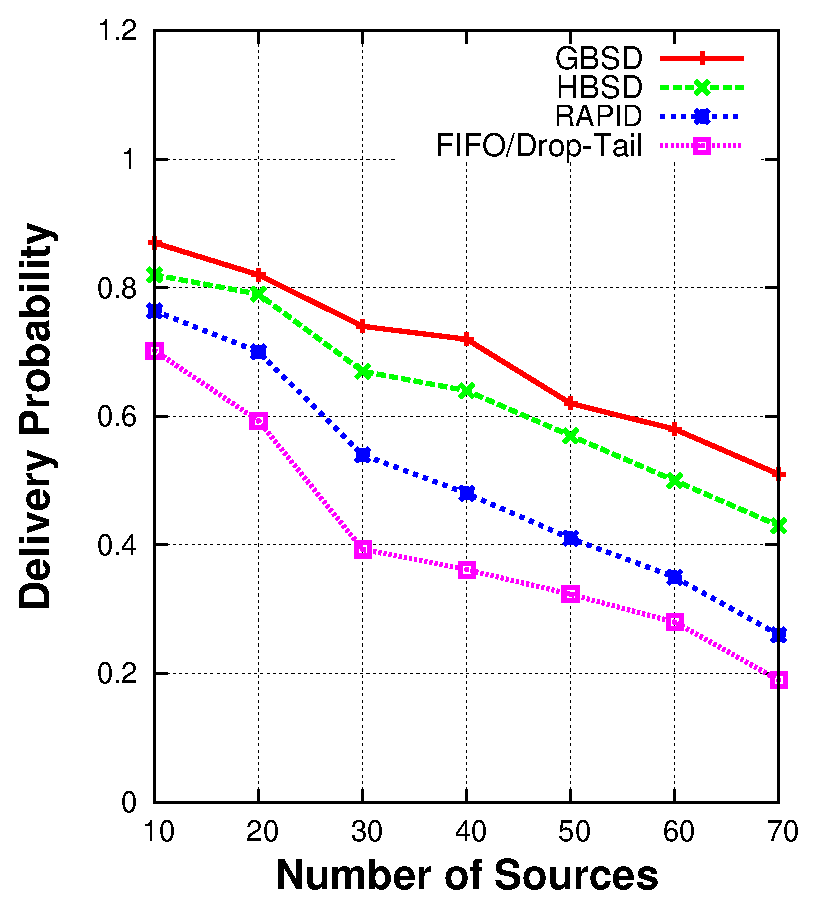
\includegraphics[width=3in,height=2.2in]{Chapitre3/fig2.eps}
\small
\caption{Delivery Probability for Epidemic Routing with different scheduling and drop policies (both buffer and bandwidth constraints).}\normalsize
\label{DR-RWP}
\end{figure}

\begin{figure}[!h]
\centering
\includegraphics[width=3in,height=2.2in]{Chapitre3/fig22.eps}
\small
\caption{Delivery Probability (KAIST mobility trace).}
\normalsize
\label{DR-KAIST}
\end{figure}

\begin{table}[!h]
\renewcommand{\arraystretch}{1.1}
\caption{Taxi Trace \& Limited buffer and bandwidth}
\centering
\footnotesize
\begin{tabular}{|p{2.5cm}||p{0.9cm}||p{0.9cm}||p{0.9cm}||p{1.5cm}|}
\hline
\bfseries Policy: & GBSD & HBSD & RAPID & FIFO\textbackslash DT\\
\hline\hline
D. Probability:&0.72 &0.66 &0.44 &0.34\\
\hline\hline
D. Delay(s):&14244&15683&20915&36412\\
\hline
\end{tabular}
\label{T-LB+LB}
\end{table}

\begin{table}[!h]
\renewcommand{\arraystretch}{1.1}
\caption{ZebraNet Trace \& Limited buffer and bandwidth}
\centering
\footnotesize
\begin{tabular}{|p{2.5cm}||p{0.9cm}||p{0.9cm}||p{0.9cm}||p{1.5cm}|}
\hline
\bfseries Policy: & GBSD & HBSD & RAPID & FIFO\textbackslash DT\\
\hline\hline
D. Probability:&0.68&0.59&0.41&0.29\\
\hline\hline
D. Delay(s):&4306&4612&6705&8819\\
\hline
\end{tabular}
\label{ZebraNetResults}
\end{table}


\begin{table}[!h]
\renewcommand{\arraystretch}{1.1}
\caption{HCMM Trace (70 CBR sources)}
\centering
\footnotesize
\begin{tabular}{|p{1.8cm}|p{0.9cm}|p{0.9cm}|p{0.9cm}|p{1.5cm}|}
\hline
\bfseries Policy: & GBSD & HBSD & RAPID & FIFO\textbackslash DT\\
\hline
D. Probability:&0.62&0.55&0.38&0.23\\
\hline
D. Delay(s):&3920&4500&6650&8350\\
\hline
\end{tabular}
\label{HCMM-Results}
\end{table}

Figure~\ref{DR-RWP} shows the delivery rate based on the Random Waypoint model. From this plot, it can be seen that: the GBSD policy plugged into Epidemic routing gives the best performance for all numbers of sources. When congestion-level decreases, so does the difference between GBSD and other protocols, as expected. Moreover, the HBSD policy also outperforms existing protocols (RAPID and Epidemic based on FIFO/drop-tail) and performs very close to the optimal GBSD. Specifically, for $70$ sources, HBSD offers an almost 60\% improvement in delivery rate compared to RAPID and is only 14\% worse than GBSD. Similar conclusions can be also drawn for the case of the real Taxi trace,  ZebraNet trace, KAIST trace or the HCMM model and $70$ sources. Results for these cases are respectively summarized in Table~\ref{T-LB+LB}, Table~\ref{ZebraNetResults}, Figure~\ref{DR-KAIST} and Table~\ref{HCMM-Results}.

\subsection{Performance evaluation for delivery delay}
\label{sec:sims:DD}

To study delays, we increase messages' TTL (and simulation duration), to ensure almost every message gets delivered, as follows. Random Waypoint: (duration 10.5h, TTL = 1.5h). ZebraNet: (simulation duration = 28h, TTL = 4h). Taxi trace:  (simulation duration = 84h, TTL = 12h). Traffic rates are as in Section~\ref{sec:sims:DR}.

\begin{figure}[!h]
\centering
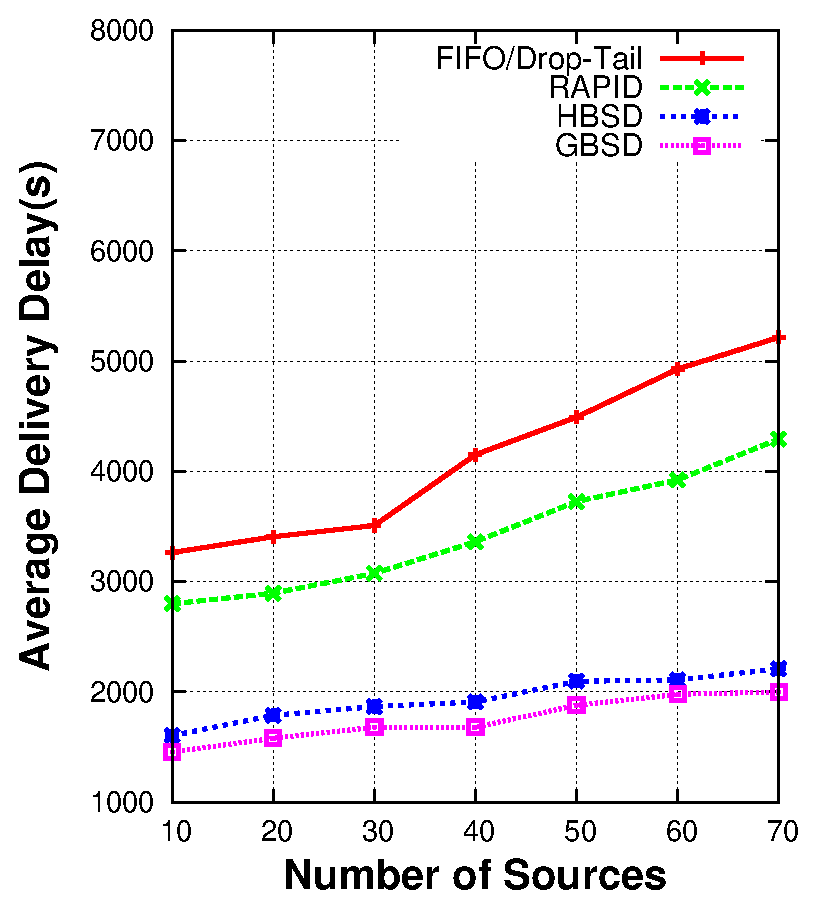
\includegraphics[width=3in,height=2.2in]{Chapitre3/fig3.eps}
\caption{Delivery Delay for Epidemic Routing with different scheduling and drop policies (both buffer and bandwidth constraints).}
\label{DD-RWP}
\end{figure}

\begin{figure}[!h]
\centering
\includegraphics[width=3in,height=2.2in]{Chapitre3/fig33.eps}
\caption{Delivery Delay (KAIST mobility trace).}
\label{DD-KAIST}
\end{figure}

For the random waypoint mobility scenario, Figure~\ref{DD-RWP} depicts the average delivery delay for the case of both limited buffer and
bandwidth. As in the case of delivery rate, GBSD gives the best performance for all considered scenarios. Moreover, the HBSD policy
outperforms the two routing protocols (Epidemic based on FIFO/drop-tail, and RAPID) and performs close to GBSD. Specifically,
for 70 sources and both limited buffer and bandwidth, HBSD average delivery delay is 48\% better than RAPID and only 9\% worse than
GBSD.

Table~\ref{T-LB+LB}, Table~\ref{ZebraNetResults}, Figure~\ref{DD-KAIST} and Table~\ref{HCMM-Results} show that similar conclusions can be drawn for the delay under respectively the real Taxi(s), ZebraNet trace, KAIST trace and the HCMM model. 

\subsection{Optimality}
\label{GBSD:Optimality}

\begin{figure}[!h]
\centering
\includegraphics[width=3in,height=2.2in]{Chapitre3/AvgDistancePerCoordinate.eps}
\caption{Normalized Manhattan distance between two consecutive N optimal vectors.}
\label{Sensitivity}
\end{figure}

\begin{figure}[!h]
\centering
\includegraphics[width=3in,height=2.2in]{Chapitre3/NbrCopiesDiff.eps}
\caption{Difference in terms of Nbr of copies.}
\label{DiffinTermsOfNbrCopies}
\end{figure}

Here, we use simulations results (based on the RW scenario) that our proposed policy (GBSD) can ``keep up'' with the optimal algorithm described in Section~\ref{OptimalityOfGradientPolicy}. Figure~\ref{Sensitivity} plots the normalized Manhattan distance $d(X,Y) = \frac{\sum_{i=1}^{K}|x_i - y_j|}{K}$ between two consecutive optimal copy vectors, resulting from solving the optimal centralized version offline. These optimal vectors are calculated every $4ms$, corresponding to the average time between any two consecutive contacts among the network. As is evident in the figure, this distance is very small, implying that our distributed gradient-ascent implementation of this policy (GBSD/HBSD) has enough time to converge to the optimal vector, before this changes significantly. In order to further validate the optimality of our policy, we compare in Figure~\ref{DiffinTermsOfNbrCopies} the absolute difference between the number of copies assigned to a message by our GBSD policy and the number of copies allocated to the same message by the optimal algorithm~\ref{OptimalityOfGradientPolicy}. We have picked some messages randomly and plot this difference along a time window in their lifetime. These results show that the GBSD policy stays is able to follow the optimal one with an average error of $1-2$ copies allocated at most. We believe this result consolidates the optimality properties of our proposed distributed implementation of the optimal policy.

\section{Maintaining Network History}
\label{sec:NetworkHistory}

The results of the previous section clearly show that our distributed policy (HBSD) that uses estimators of global message state (rather than actual state) successfully approximates the performance of the optimal policy (GBSD). This is as an important step towards a practical implementation of efficient buffer management and scheduling algorithms on wireless devices. Nevertheless, in order to derive good estimators in a distributed manner, nodes need to exchange (a possibly large amount of) metadata during every node meeting. Potentially, each node needs to know the history of all messages having passed through a node's buffer, for every node in the network. In a small network, the amount of such ``control'' data might not be much, considering that large amounts of data transfers can be achieved between 802.11 transceivers during short contacts (data transfers of a few $10s$ of MBytes have been reported for experiments between vehicles moving at high speeds~\cite{Keshav:Mobisys07}). Nevertheless, in larger networks, this method can quickly become unsalable and interfere with (or starve) data transmissions, if statistics maintenance and collection is naively done.

In this section, we describe the type of statistics each node maintains towards calculating the HBSD utility for each message, and propose a number of mechanisms and optimizations to significantly reduce (and control) the amount of metadata exchanged during contacts. Finally, we explore the impact of reducing the amount of collected statistics on the performance of our buffer management and scheduling policy. Our results suggest that, with a carefully designed statistics collection and maintenance scheme, order(s) of magnitude less metadata can be exchanged (compared to maintaining a complete view about the network), without significantly affecting performance.

\subsection{Maintaining Buffer State History}
\label{NetworkHistoryModel}

In order to keep track of the statistics about past messages necessary to assign appropriate utility values to messages considered for transmission or dropping, we propose that each node maintains the data structure depicted in Figure~\ref{NHM}. Each node maintains a list of messages whose history in the network it keeps track of (we will see in the next section how a node chooses which messages to include in this list). For each message, it maintains its $ID$ (a unique string resulting from the combination of some of its attributes), its $TTL$ and the list of nodes that have \emph{seen} it before (i.e. had stored the messages at some time in the past and should be accounted towards calculating $m$ or $n$). Then, for each of the nodes in the list, it maintains a data structure with the following data: (i) the node's $ID$, (ii) a boolean array $Copies\_Bin\_Array$, and (iii) the version $Stat\_Version$ associated to this array.

The $Copies\_Bin\_Array$ array (Figure~\ref{BA}) enables nodes to maintain dynamically what each message experienced during its life time. For a given entry pair (message $a$ and node $b$) in this list, the $Copies\_Bin\_Array[k]$ indicates if the node $a$ had already stored or not a copy of message $b$ in its buffer during \emph{Bin} $k$. In other words, time is quantized into ``bins'' of size $Bin\_Size$, and bin $k$ correspond to the period of time between $k*Bin\_Size$ and $(k+1)*Bin\_Size$. As a result, the size of the $Copies\_Bin\_Array$ is equal to $TTL/Bin\_Size$.

How should one choose $Bin\_Size$? Clearly, the larger it is, the fewer the amount of data a node needs to maintain and to exchange during each meeting; however, the smaller is also the granularity of values the utility function can take and thus the higher the probability of an incorrect (scheduling or buffer management) decision. As already described in Section~\ref{sec:optimal-policy}, message transmissions can occur only when nodes encounter each other. This is also the time granularity at which buffer state changes occur. Hence, we believe that a good trade-off is to monitor the evolution of each message's state at a bin granularity in the order of meeting times. This \emph{already results in a big reduction of the size of statistics to maintain locally} (as opposed to tracking messages at seconds or milliseconds granularity), while still enabling us to infer the correct messages statistics. Note that  according to the \emph{Nyquist-Shannon}~\cite{Nyquist} sampling theorem, a good approximation of the size of a \emph{Bin} would be equal to inter-meeting-time/2. A running average of the observed times between consecutive meetings could be maintained easily, in order to dynamically adjust the bin size~\cite{akis:ton-multi}. 

Finally, the $Stat\_Version$ indicates the Bin at which the last update occurred. Let's assume that a message $a$ is first stored at a node $b$ during bin $3$. It then creates a new entry in its list for pair ($a$,$b$), inserts $0$s in bins $0-2$ of the new $Copies\_Bin\_Array$ and $1$s in the rest of the bins, and sets the $Stat\_Version$ to $3$. If later, at in bin $5$ node $b$ decides to drop this message, then the list entry is maintained, but it sets all bins from $5$ to $TTL/Bin\_Size$ to $0$, and updates the $Stat\_Version$ to $5$. Finally, when the TTL for message $a$ elapses (regardless of whether $a$ is still present in $b$'s buffer or not), $b$ sets the $Stat\_Version$ to $TTL/Bin\_Size$, which also indicates that all information about the history of \emph{this} message in \emph{this} buffer is now available. The combination of how the $Copies\_Bin\_Array$ is maintained and the $Stat\_Version$ updated, ensures that only the minimum amount of necessary metadata \emph{for this pair of (message, node)} is exchanged during a contact.

We note also that, in principle, a $Message\_Seen\_Bin\_Array$ could be maintained, indicating if a node $a$ had \emph{seen} (rather than \emph{stored} a message $b$ at time $t$, in order to estimate $m(T)$. However, it is easy to see that the $Message\_Seen\_Bin\_Array$ can be deduced directly from the $Copies\_Bin\_Array$, and thus no extra storage is required.
Summarizing, based on this lists maintained by all nodes, any node can retrieve the vectors $N(T)$ and $M(T)$ and can calculate the HBSD per-message utilities described in Section~\ref{sec:learning} without a need for an \emph{oracle}.

\subsection{Collecting Network Statistics}
\label{NHCM}

We have seen so far what types of statistics each node maintains about each past (message ID, node ID) tuple it knows about. Each node is supposed to keep up-to-date the statistics related to the messages it stores locally (i.e. entries in the list of Figure~\ref{NHM} corresponding to its own node ID). However, it can only update its knowledge (and the respective entry) about the state of a message $a$ at a node $b$ when it either meets $b$ directly, or it meets a node that has more recent information about the ($a$, $b$) tuple (i.e. a higher $Stat\_Version$). The goal of the statistics collection method is that, through such message exchanges, nodes converge to a unified view about the state of a given message at \emph{any} buffer in the network, during its lifetime.

\emph{Sampling Messages to Keep Track of:} We now look in more detail into what kind of metadata nodes should exchange. The first interesting question is the following: \emph{should a node maintain global statistics for \emph{every} message it has heard of or only a subset?} We argue that monitoring a dynamic subset of these messages is sufficient to quickly\footnote{While speed of convergence is not that important, due to our history-based approach, it becomes significant in non-stationary scenarios with traffic load fluctuations and node churn, as we shall see.} converge to the correct expectations we need for our utility estimators. This dynamic subset is illustrated in Figure~\ref{SE} as being the Messages Under Monitoring, which are stored in the \emph{MUM} buffer; it is dynamic because its size is kept fixed while messages inside it change. When a node decides to store a message for the first time, if there is space in its MUM buffer, it also inserts it there and will track its global state.  In other words, each node randomly chooses a few messages it will \emph{sample}, for which it will attempt to collect global state, and does not keep track of all messages currently alive in the network. The actual \emph{sampling rate} depends on the size of the MUM buffer and the offered traffic load, and results in significant further reduction in the amount of metadata exchanged. At the same time, a smaller MUM buffer might result to slower convergence (or even lack of). In Section~\ref{PENHCM} we study the impact of MUM buffer size on the performance of our algorithm.

\emph{Handling Converged Messages:} Once the node collects an entire history of a given message, it removes it from the \emph{MUM} buffer and pushes it to the buffer of Messages with a Complete History (\emph{MCH}). A node considers that it has the complete history of a given message only when it gets the last version (i.e. $Stat\_Version = TTL/Bin\_Size$) of the statistics entries related to all the nodes the message goes through during its $TTL$. Note that there is a chance that a node might ``miss'' some information about a message it pushes in its MCH. This occurs, for example, if it receives the last version for a subset of nodes which had the message, before it receives \emph{any} version from another node that also had the message. This probability depends on the statistics of the meeting time (first and second moment) and the TTL value. Nevertheless, for many scenarios of interest, this probability is small and it may only lead to slightly underestimating the $m$ and $n$ values. Finally, note that, once a node decides to move a message to the \emph{MCH} buffer, it only needs to maintain a short summary (i.e. number of nodes with a copy $n(T)$ and number of nodes having seen the message, $m(T)$, at time $T$) rather than the per node state as in  Figure~\ref{NHM}.

\emph{Statistics Exchanged:} Once a contact opportunity is present, both peers have to ask only for newer versions of the statistics entries (message ID, node ID) related to the set of messages buffered in their \emph{MUM} buffer. This ensures that, even for the sampled set of messages, only new information is exchanged and no bandwidth is wasted. This optimization does not introduce any extra latency in the convergence of our approximation scheme.


\begin{figure}[!h]
\centering
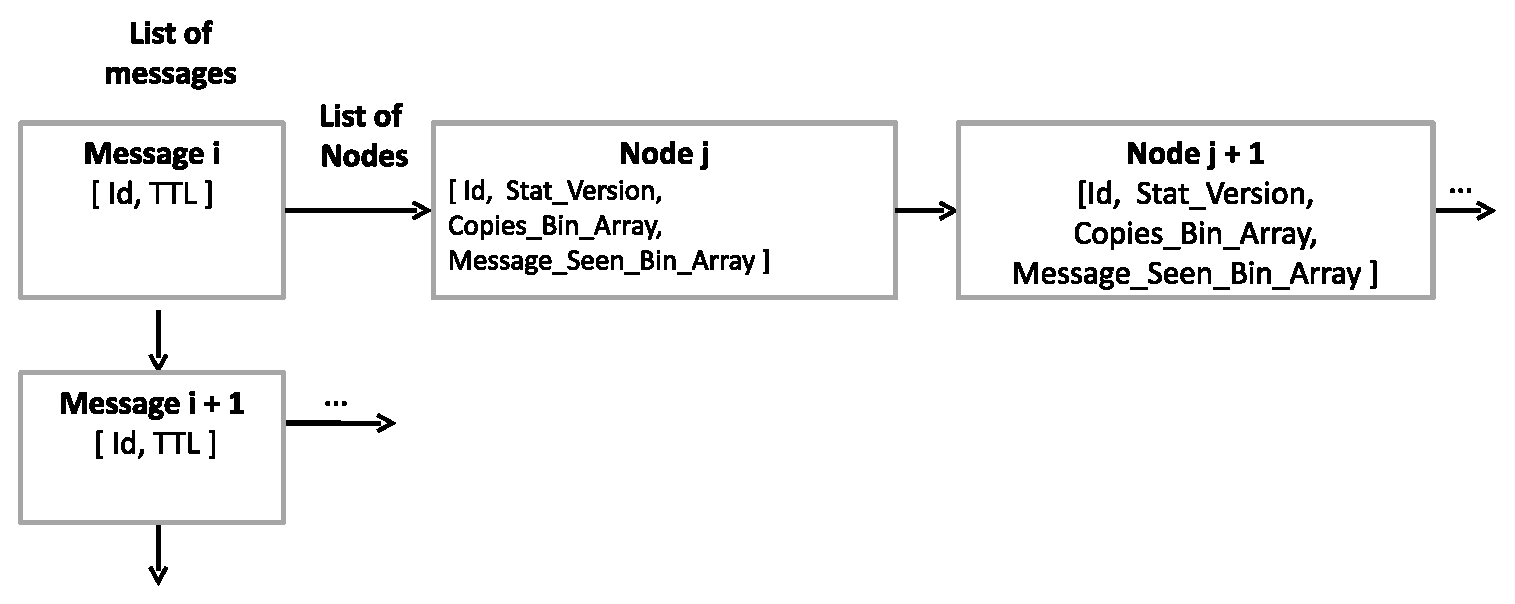
\includegraphics[width=3in,height=2in]{Chapitre3/Stat_Matrix.eps}
\caption{Network History Data Structure}
\label{NHM}
\end{figure}
\begin{figure}
\centering
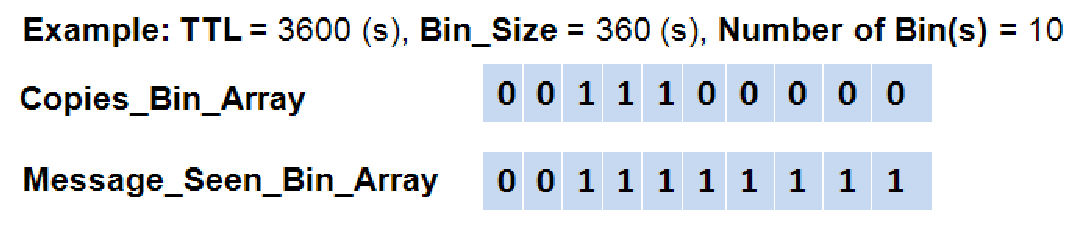
\includegraphics[width=2.5in,height=0.7in]{Chapitre3/Bin_Array.eps}
\caption{Example of Bin arrays}
\label{BA}
\end{figure}

\begin{figure}[!h]
\centering
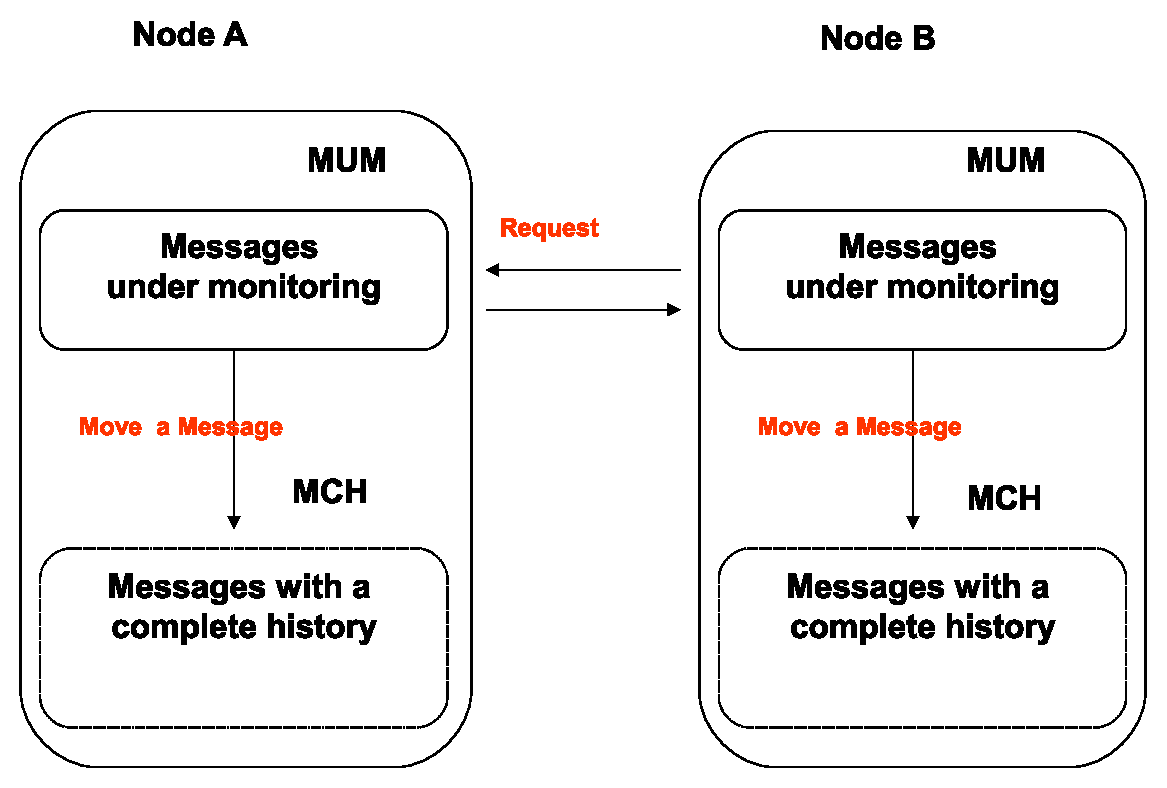
\includegraphics[width=2.5in,height=1.6in]{Chapitre3/StatisticsExchanging.eps}
\caption{Statistics Exchange and Maintenance.}
\label{SE}
\end{figure}

\subsection{Performance Tradeoffs of Statistics Collection}
\label{PENHCM}

We have presented a number of optimizations to (considerably) reduce the amount of metadata stored and the amount of signalling overhead. Here, we explore the trade-off between the signalling overhead, its impact on performance, and the dynamicity of a given scenario. Our goal is to identify operation points where the amount of signalling overhead is such that it interferes minimally with data transmission, while at the same time it suffices to ensure timely convergence of the required utility metrics per message. We will consider throughout the random waypoint simulation scenario described in Section~\ref{sec:sims:DR}. We have observed similar behaviour for the trace-based scenarios.

\textbf{Amount of Signalling Overhead per Contact:} We start by studying the effect of varying the size of the \emph{MUM} buffer (number of messages under monitoring) on the average size of exchanged statistics per-meeting. Figure~\ref{StatOverhead} compares the average size of statistics exchanged during a meeting between two nodes for three different sizes of the \emph{MUM} buffer (20, 50 and 80), as well as for the basic epidemic statistics exchange method (i.e. unlimited MUM). We vary the number of sources in order to cover different congestions regimes.

Our first observation is that increasing the traffic load (and thus the amount of congestion) results in decreasing the average amount of statistics exchanged per-meeting (except for the MUM size of 20 messages). This might be slightly counterintuitive, since a higher traffic load implies more messages to keep track of. However, note that a higher congestion level also implies that much fewer copies per message will co-exist at any time (and new versions are less frequently created). As a result, much less metadata per message is maintained and exchanged, resulting in a downward trend. In the case of a MUM size of $20$, it seems that these two effects balance each other out. In any case, the key property here is that, in contrast with the flooding-based method of~\cite{Levine:Sigcomm07}, \emph{our distributed collection method scales well, not increasing the amount of signalling overhead during high congestion.}

A second observation is that, using our statistics collection method, a node can reduce the amount of signalling overhead per meeting up to an order of magnitude (e.g. for MUM = 20), compared to the unlimited MUM case, even in this relatively small scenario of $70$ nodes. (Note also that, the plot shown for the epidemic case, already implements the binning and versioning optimizations of Section~\ref{NetworkHistoryModel}).)

\begin{figure}[!h]
\centering
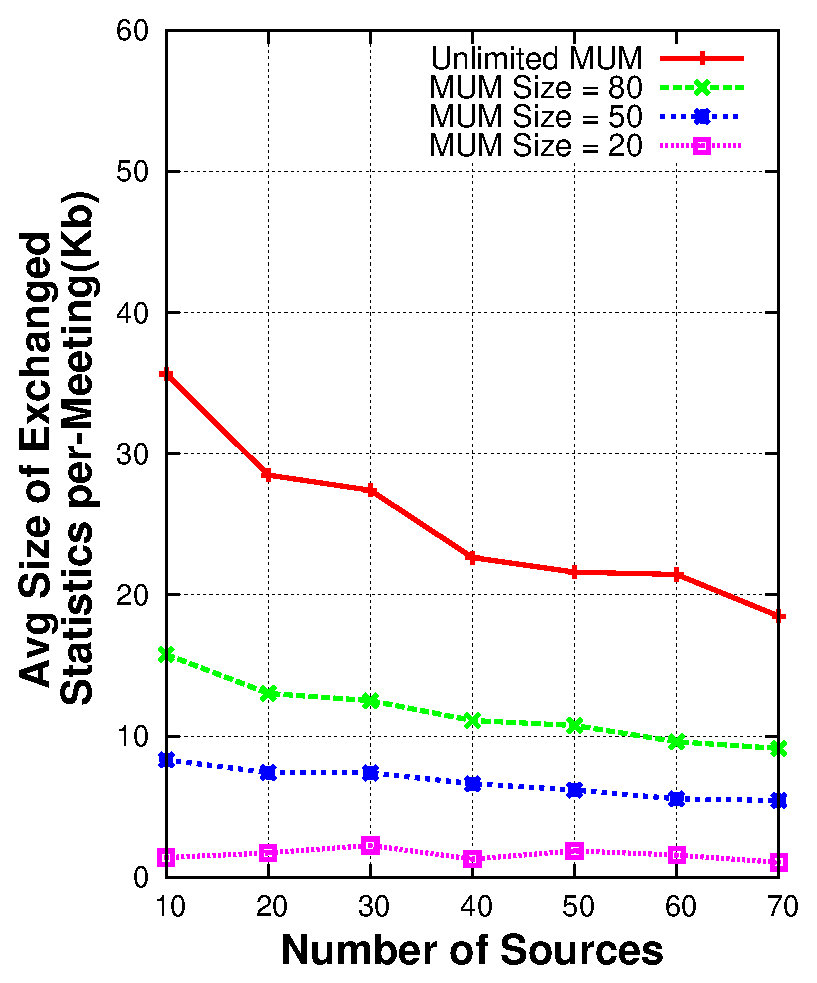
\includegraphics[width=3in,height=2.2in]{Chapitre3/fig7.eps}
\caption{Signalling overhead (per contact) resulting from HBSD statistics collection.}
\label{StatOverhead}
\end{figure}

Finally, we plot in Figure~\ref{PMED} the average size of exchanged (non-signalling) data per-meeting. We can observe that increasing the size of the \emph{MUM} buffer results in a slight decrease of the data exchanged. This is due to the priority we give to statistics exchange during a contact. We note also that this effect becomes less pronounced when congestion increases (in line with Figure~\ref{StatOverhead}). Finally, in the scenario considered, we can observe that, for MUM sizes less than $50$, signalling does not interfere with data transmissions (remember that packet size is 5KB). This suggests that, in this scenario, a MUM size of 50 messages represents a good choice with respect to the resulting signalling overhead. In practice, a node could find this value online, by dynamically adjusting its MUM size and comparing the resulting signalling overhead with average data transfer. It is beyond the scope of this work to propose such an algorithm. Instead, we are interested in exposing the various tradeoffs and choices involved in efficient distributed estimation of statistics. Towards this goal, we explore next the effect of the MUM sizes considered on the performance of our HBSD algorithm.


\begin{figure}[!h]
\centering
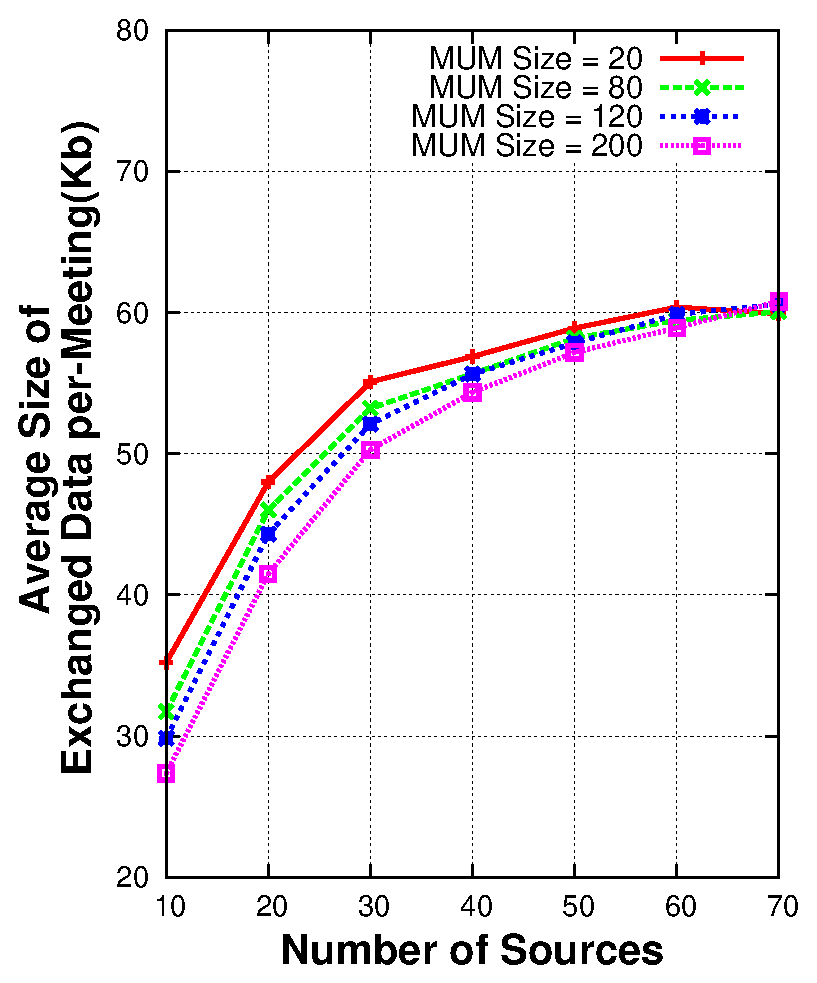
\includegraphics[width=3in,height=2.2in]{Chapitre3/fig8.eps}
\caption{Average size of exchanged (non-signalling) data per contact.}
\label{PMED}
\end{figure}

\textbf{Convergence of Utilities and Performance of the HBSD Policy :} In this last part, we fix the number of sources to $50$ and we look at the impact of the size of the \emph{MUM} buffer on (i) the time it takes the HBSD delivery rate utility to converge, and (ii) its accuracy. We use the \emph{mean relative square error} to measure the accuracy of the HBSD delivery rate utility, defined as follows:

\begin{eqnarray*}
\frac{1}{\# Bins}* \sum_{Bins}^{}\frac{(A-B)^2}{B^2},
\end{eqnarray*}

where, for each \emph{bin}, $A$ is the estimated utility value of Eq. (\ref{HBSD-DR-U}) (calculated using the approximate values of $m$ and $n$, collected with the method described previously) and $B$ is the utility value calculated using the real values of $m$ and $n$.

\begin{figure}[!h]
\centering
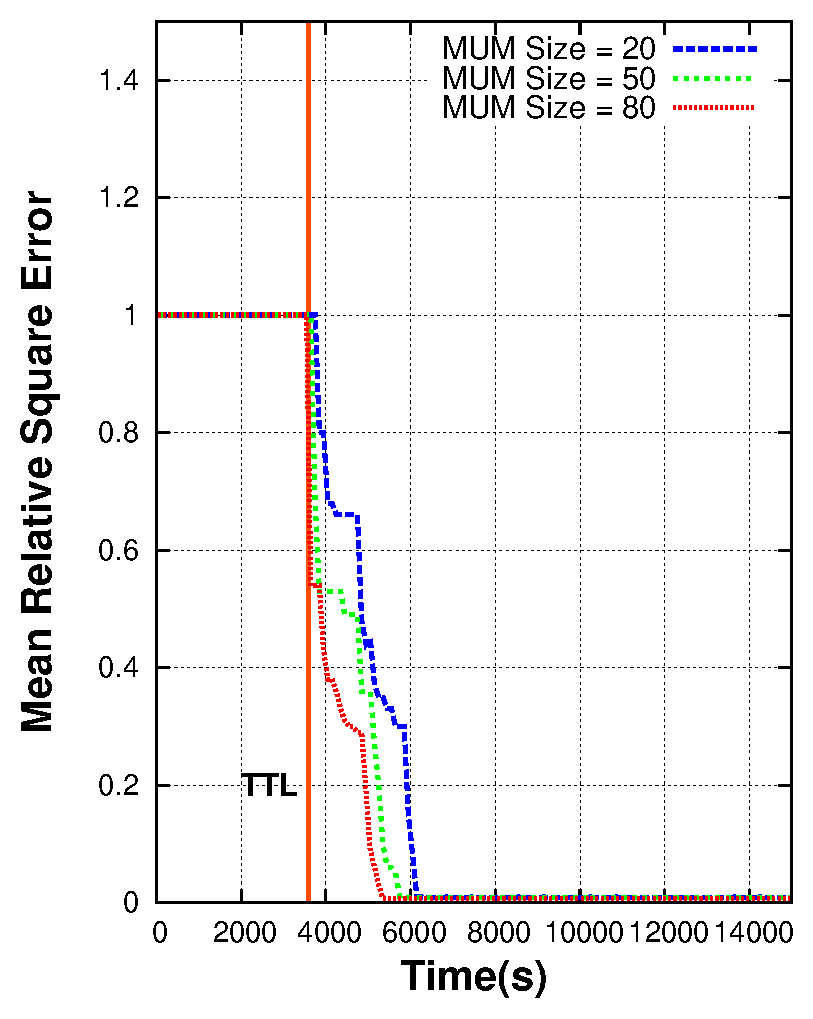
\includegraphics[width=3in,height=2.2in]{Chapitre3/fig9.eps}
\caption{Mean relative square errors for HBSD delivery rate utility.}
\label{DR-RE}
\end{figure}

Figure~\ref{DR-RE} plots the \emph{mean relative square errors} for the HBSD delivery rate utility, as a function of time. We can observe that, increasing the size of the \emph{MUM} buffer results in faster reduction of the \emph{mean relative square error} function. With a \emph{MUM} buffer of $80$ messages, the delivery rate utility estimate converges $800$ seconds faster than using an \emph{MUM} buffer of $20$ messages. Indeed, the more messages a node tracks in parallel, the faster it can collect a working history of past messages that it can use to calculate utilities for new messages considered for drop or transmission. We observe also that all plots converge to the same very small error value~\footnote{We speculate that this remaining error might be due to slightly underestimating m and n, as explained earlier.}. Note also that it is not the absolute value of the utility function (during different time bins) that we care about, but rather the \emph{shape} of this function, whether it is increasing or decreasing, and the relative utility values. (We will look into the shape of this function at different congestion regimes in the next section.)

In fact, we are more interested in the end performance of our HBSD, as a function of how ``aggressively'' nodes collect message history. In Figures~\ref{HBSD-AVG-DR-MUM} and~\ref{HBSD-AVG-DD-MUM}, we plot the delivery rate and delay of HBSD, respectively, for different MUM sizes. These results correspond to the scenario described in Section~\ref{sec:sims:DR}, where we have a fixed number of CBR sources. As is evident from these figures, regardless of the size of the \emph{MUM} buffer sizes, nodes eventually gather enough past message history to ensure an accurate estimation of per message utilities, and a close-to-optimal performance. In such scenarios, where traffic intensity is relatively stable, even a rather small MUM size (i.e. very low sampling rate) suffices to achieve good performance. This is not necessarily the case when traffic load experiences significant fluctuations (e.g. due to new popular content appearing in the network).

\begin{figure}[!h]
  \begin{center}
    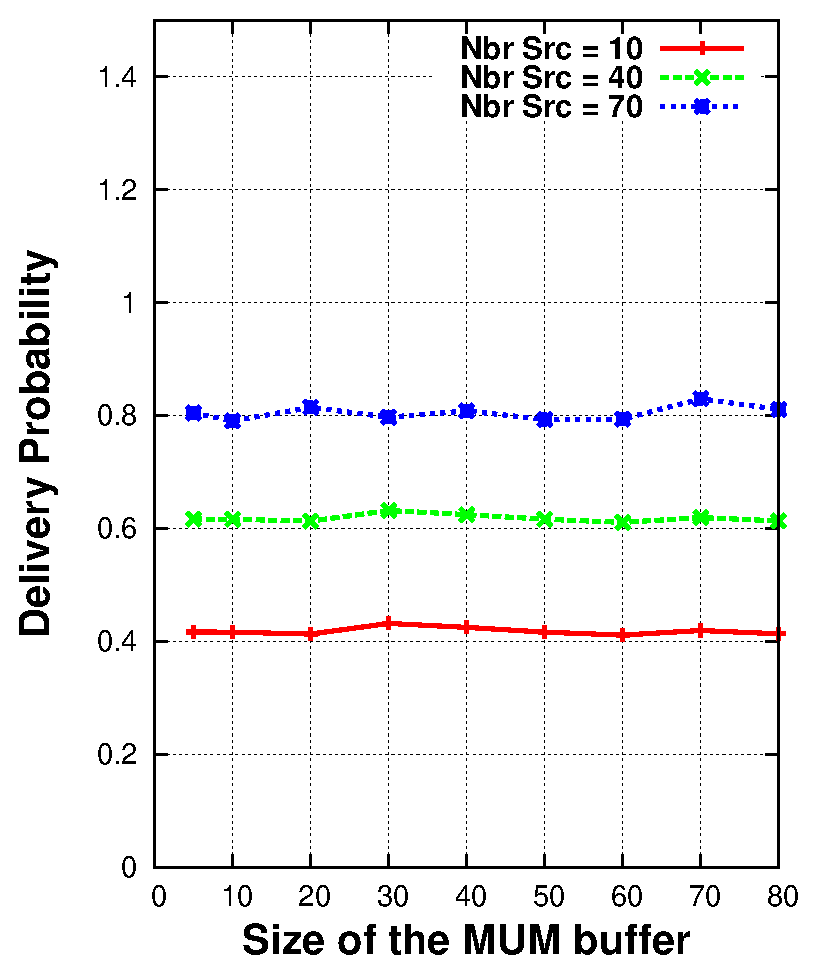
\includegraphics[width=3in,height=2.2in]{Chapitre3/fig13.eps}
  \end{center}
  \caption{Delivery Probability for HBSD with statistics collection (static traffic load).}
  \label{HBSD-AVG-DR-MUM}
\end{figure}

\begin{figure}[!h]
  \begin{center}
    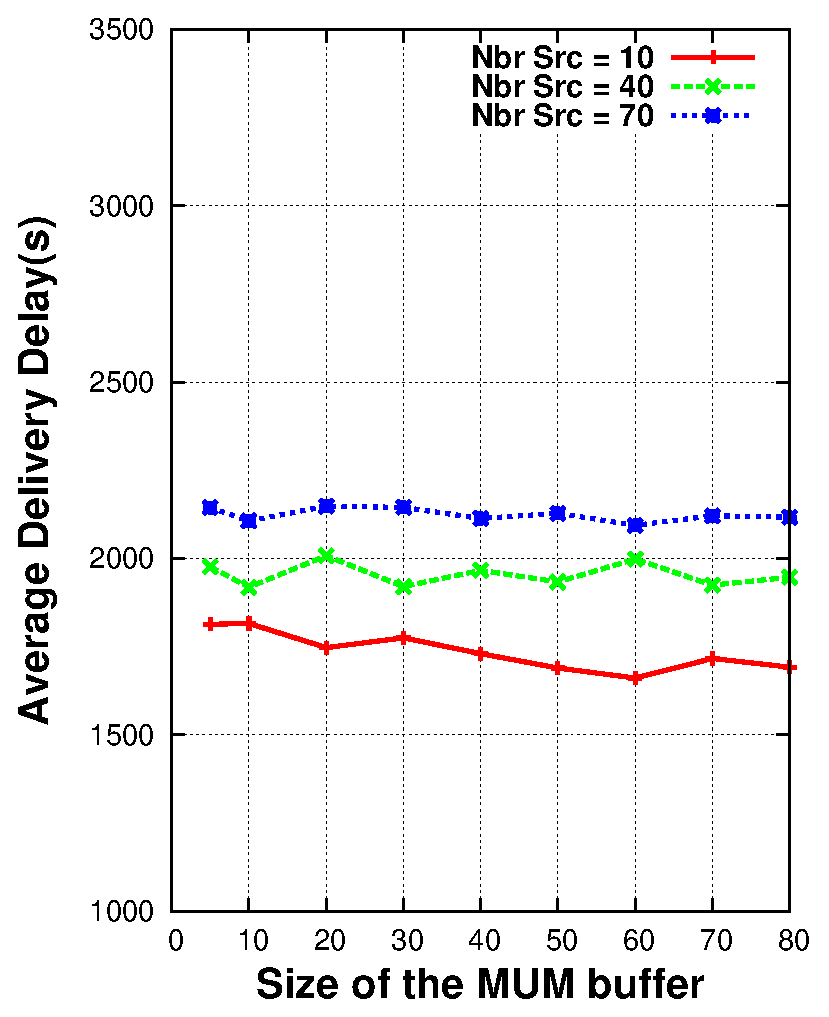
\includegraphics[width=3in,height=2.2in]{Chapitre3/fig14.eps}
  \end{center}
  \caption{Deliver Delay for HBSD with statistics collection (static traffic load).}
  \label{HBSD-AVG-DD-MUM}
\end{figure}

When the offered traffic load changes frequently (or node churn is high, e.g. experiencing ``flash crowds''), convergence speed becomes important. The bigger the \emph{MUM} buffer the faster our HBSD policy react to changing congestion levels. We illustrate this with the following experiment. We maintain the same simulation scenario, but we vary the number of CBR sources among each two consecutive TTL(s), from $10$ to $70$ sources (i.e. the first and second TTL window we have $10$ sources, the third and fourth window $70$ sources, etc. --- this is close to a \emph{worst case} scenario, as there is a sevenfold increase in traffic intensity within a time window barely higher than a TTL, which is the minimum required interval to collect any statistics). Furthermore, to ensure nodes use non-obsolete statistics towards calculating utilities, we force nodes to apply a \emph{sliding window} of one \emph{TTL} to the messages with complete history stored in the \emph{MCH} buffer, and to delete messages out of this \emph{sliding window}\footnote{A running average could be used for smoother performance. We only care here to demonstrate the effect of dynamic traffic loads.}

Figures~\ref{HBSD-AVG-DR-DYNAMIC} and~\ref{HBSD-AVG-DD-DYNAMIC} again plot the HBSD policy delivery rate and delay, respectively, as a function of MUM buffer size. Unlike the constant load case, it is easy to see there that, increasing the size of the \emph{MUM} buffer, results in considerable performance improvement. Nevertheless, even in this rather dynamic scenario, nodes manage to keep up and produce good utility estimates, with only a modest increase on the amount of signalling overhead required.

\begin{figure}[!h]
  \begin{center}
    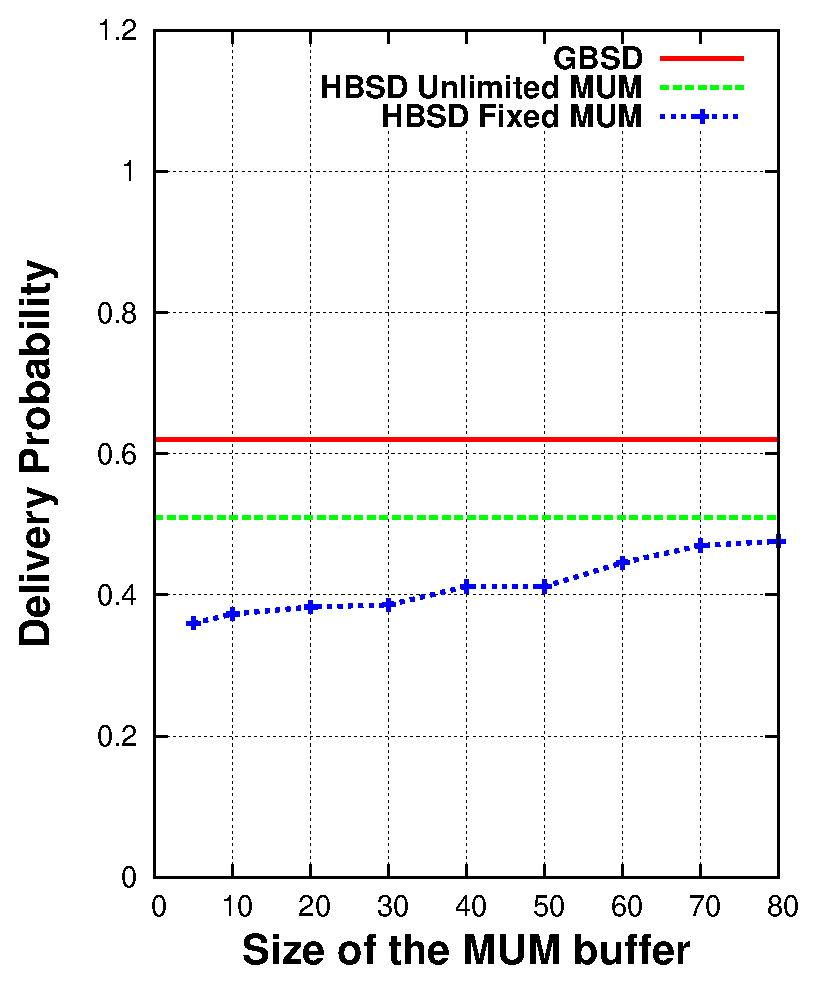
\includegraphics[width=3in,height=2.2in]{Chapitre3/fig11.eps}
  \end{center}
  \caption{Deliver Probability for HBSD with statistics collection (dynamic traffic load).}
  \label{HBSD-AVG-DR-DYNAMIC}
\end{figure}

\begin{figure}[!h]
  \begin{center}
    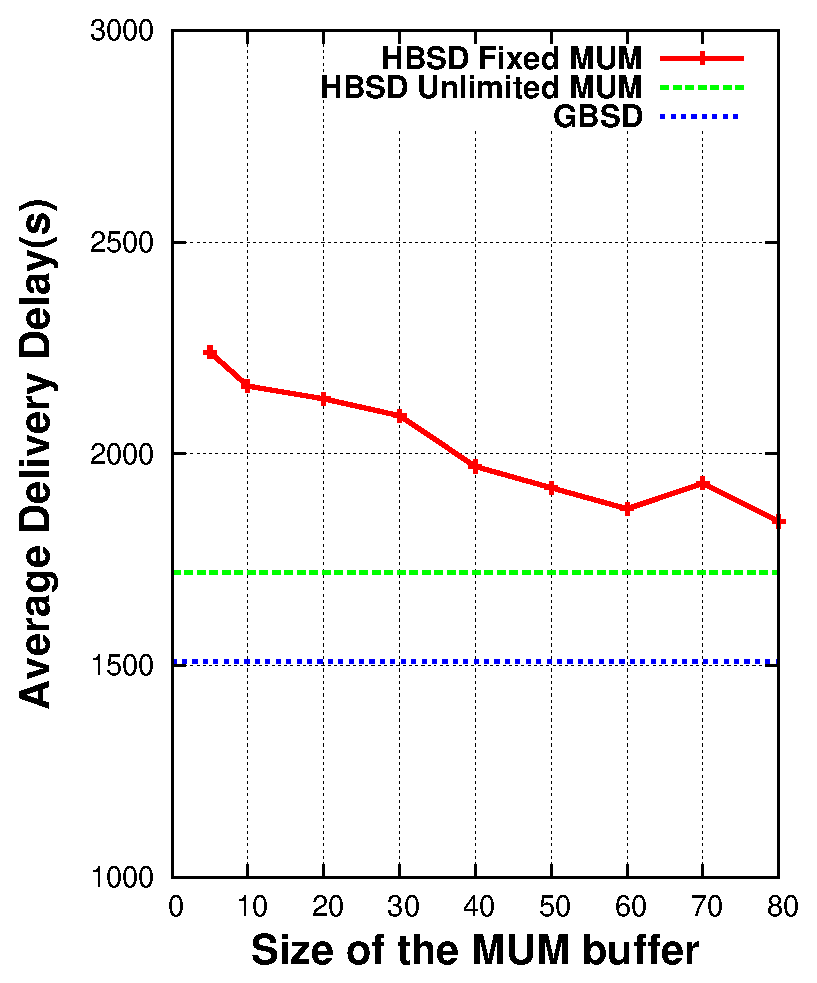
\includegraphics[width=3in,height=2.2in]{Chapitre3/fig12.eps}
  \end{center}
  \caption{Deliver Delay for HBSD with statistics collection (dynamic traffic load).}
  \label{HBSD-AVG-DD-DYNAMIC}
\end{figure}


\section{Distribution of HBSD Utilities}
\label{sec:HBSDUtilitiesDistributions}

We have described how to efficiently collect the necessary statistics in practice, and derive good estimates for the HBSD utility distribution during the lifetime of a message. In this last section, we turn our attention to the utility distributions themselves. First, we are interested whether the resulting distributions for HBSD delivery rate and delivery delay utilities react differently to different congestion levels, that is, if the priority given to messages of different ages shifts based on the offered load. Furthermore, we are interested whether the resulting utility shape (and respective optimal policy) could be approximated by simple(r) policies, in some congestion regimes.

We consider again the simulation scenario used in Section~\ref{sec:sims:DR} and Section~\ref{PENHCM}. First, we fix the number of sources to $50$, corresponding to a \emph{high congestion regime}. In Figure~\ref{HBSD-DR-HCN} and Figure~\ref{HBSD-DD-HCN}, we plot the distribution of the HBSD delivery rate and delivery delay utilities described in Sections~\ref{sec:learning:EDR} and~\ref{sec:learning:EDD}. It is evident there that the optimal utility distribution has a non-trivial shape for both optimization metrics, resulting in a complex optimal scheduling and drop policy. This also helps explain why simple drop and scheduling policies (e.g. Drop Youngest or Oldest Message, DropTail, FIFO or LIFO scheduling, etc.), considered in earlier work~\cite{Towsley:Epidemic, KrifaBS08} lead to incorrect decisions during congestion and perform worse than the GBSD and HBSD policies~\cite{KrifaBS08}.

\begin{figure}[!h]
  \begin{center}
    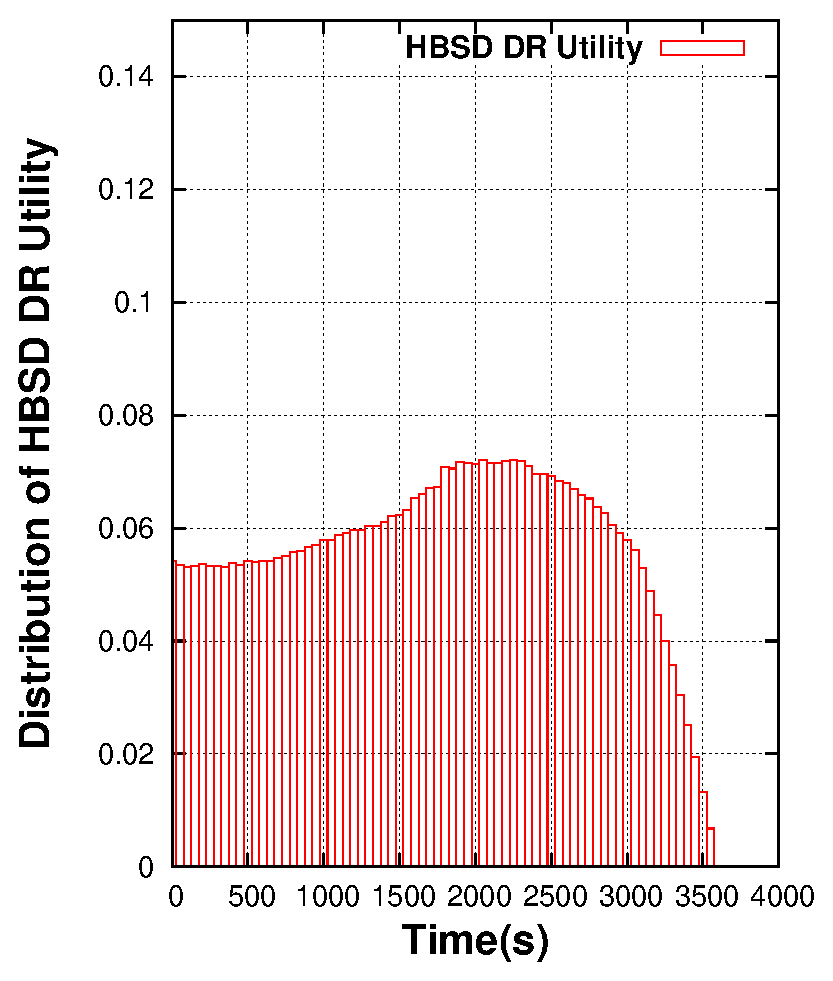
\includegraphics[width=3in,height=2.2in]{Chapitre3/fig18.eps}
  \end{center}
  \caption{Distribution of HBSD DR utility in a congested network.}
  \label{HBSD-DR-HCN}
\end{figure}

\begin{figure}[!h]
  \begin{center}
    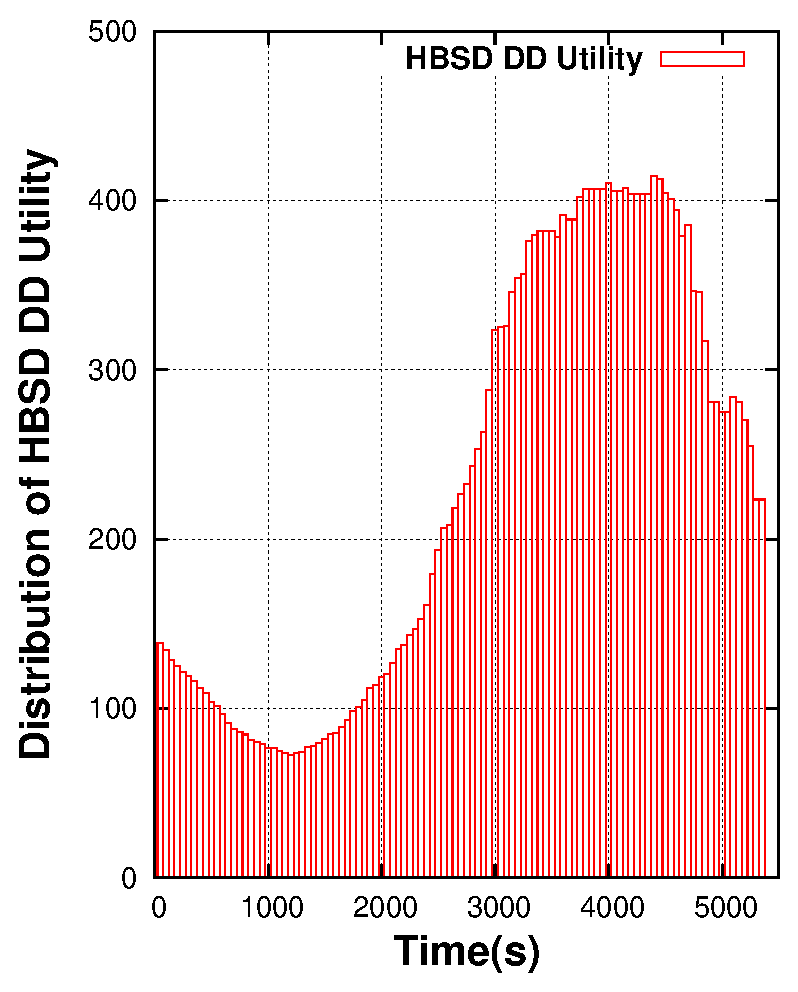
\includegraphics[width=3in,height=2.2in]{Chapitre3/fig16.eps}
  \end{center}
  \caption{Distribution of HBSD DD utility in a congested network.}
  \label{HBSD-DD-HCN}
\end{figure}

Next, we consider a scenario with low congestion. We reduce the number of sources to $15$, keep the buffer size of $20$ messages, but we also decrease the CBR rate of sources from
$10$ to $2$ messages/TTL. In Figures~\ref{HBSD-DR-LCN} and~\ref{HBSD-DD-LCN}, we plot the distribution of the HBSD delivery rate and delivery delay utilities, respectively, for this low congestion scenario. Surprisingly, our HBSD policy behaves very differently now, with both utility functions decaying monotonically as a function of time (albeit not at constant rate). This suggests that the optimal policy in low congestion regimes could be approximated by the simpler ``Drop Oldest Message'' (or schedule younger messages first) policy, which does not require any signalling and statistics collection between nodes.

To test this, in Tables~\ref{DO-HBSD-C} and~\ref{DO-HBSD-LC}, we compare the performance of the HBSD policy against a simple combination of ``Drop Oldest Message'' (for Buffer Management) and ``Transmit Youngest Message First'' (for Scheduling during a contact). We observe, that in the low congestion regime (Tables~\ref{DO-HBSD-LC}) the two policies indeed have similar performance (4\% and 5\% difference in delivery rate and delivery delay, respectively). However, in the case of a congested network (Table~\ref{DO-HBSD-C}), HBSD clearly outperforms the simple policy combination.

We can look more carefully at Figures~\ref{HBSD-DR-HCN} and~\ref{HBSD-DD-HCN}, to understand what is happening in high congestion regimes. The number of copies per message created at steady state depends on the total number of messages co-existing at any time instant, and the aggregate buffer capacity. When too many messages exist in the network (for the provided buffer space per node), uniformly assigning the available messages to the existing buffers (which is what a random drop and scheduling policy would do), would imply that every message can have only a few copies created. Specifically, for congestion higher than some level, the average number of copies per message allowed is so low that most messages cannot reach their destination during their TTL (this depends only on the number of copies and mobility model). \emph{Uniformly assigning resources between nodes is no more optimal}. Instead, to ensure that at least some messages can be delivered on time, the optimal policy gives higher priority to older messages that have managed to survive long enough (and have probably created enough copies), and ``kills'' some of the new ones being generated. This is evident by the values assigned at different bins (especially in the delivery delay case). In other words, when congestion is excessive \emph{our policy performs an indirect admission control function.}

Contrary to this, when the offered load is low enough to ensure that all messages can on average create enough copies to ensure delivery, the optimal policy simply performs a fair (i.e. equal) distribution of resources (ensured by the utility functions of Figures~\ref{HBSD-DR-LCN} and~\ref{HBSD-DD-LCN}).

\begin{table}[!h]
\renewcommand{\arraystretch}{1.1}
\caption{HBSD vs. Schedule Younger First\textbackslash Drop-Oldest in a congested network.}
\centering
\footnotesize
\begin{tabular}{|p{1.8cm}||p{2cm}||p{6cm}|}
\hline
\bfseries Policies: & HBSD & Schedule Younger First\textbackslash Drop-Oldest\\
\hline\hline
D. Rate(\%):&54&29\\
\hline\hline
D. Delay(s):&1967&3443\\
\hline
\end{tabular}
\label{DO-HBSD-C}
\end{table}

\begin{figure}[!h]
  \begin{center}
    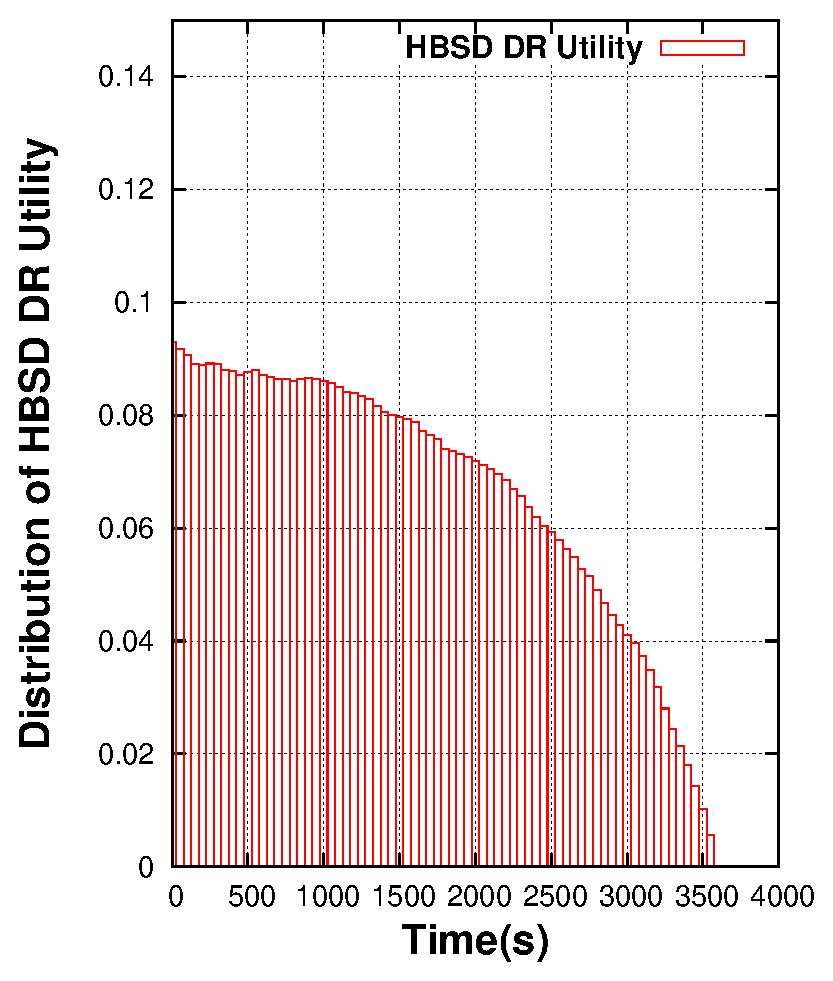
\includegraphics[width=3in,height=2.2in]{Chapitre3/fig17.eps}
  \end{center}
  \caption{Distribution of HBSD DR utility in a low congested network.}
  \label{HBSD-DR-LCN}
\end{figure}

\begin{figure}[!h]
  \begin{center}
    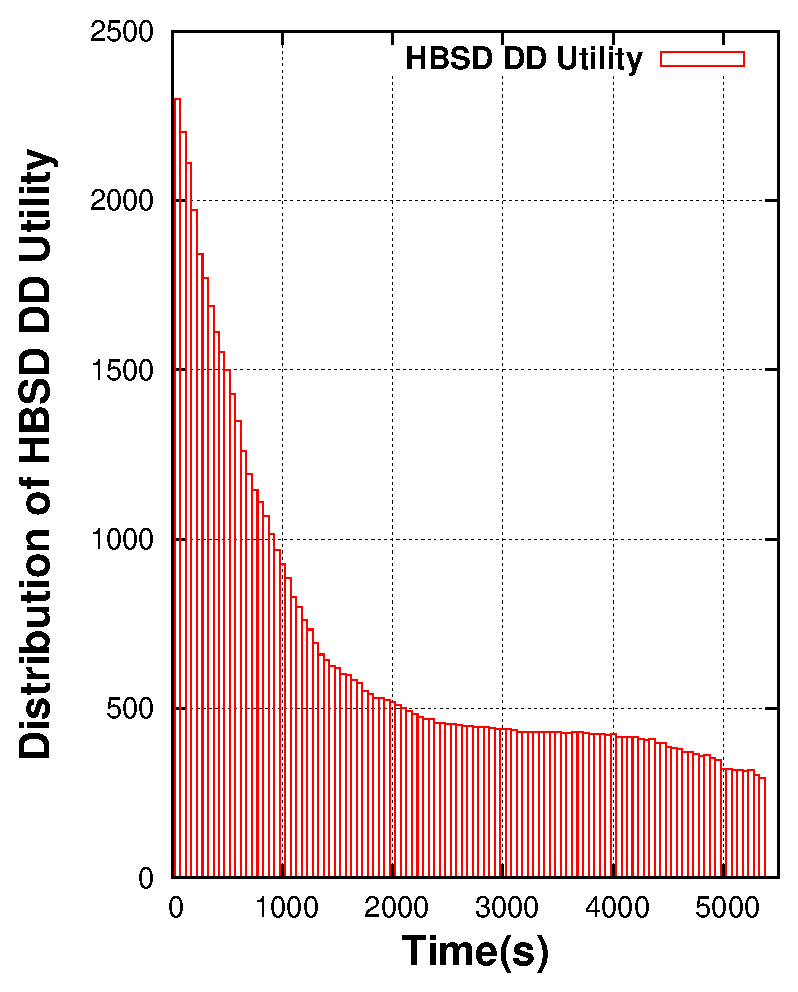
\includegraphics[width=3in,height=2.2in]{Chapitre3/fig15.eps}
  \end{center}
  \caption{Distribution of HBSD DD utility in a low congested network.}
  \label{HBSD-DD-LCN}
\end{figure}

\begin{table}[!h]
\renewcommand{\arraystretch}{1.1}
\caption{HBSD vs Schedule Younger First\textbackslash Drop-Oldest in a low congested network.}
\centering
\footnotesize
\begin{tabular}{|p{1.8cm}||p{2cm}||p{6cm}|}
\hline
\bfseries Policies: & HBSD & Schedule Younger First\textbackslash Drop-Oldest\\
\hline\hline
D. Rate(\%):&87&83\\
\hline\hline
D. Delay(s):&1530&1618\\
\hline
\end{tabular}
\label{DO-HBSD-LC}
\end{table}

The above findings suggest that it would be quite useful to find a generic way to signal the congestion level and identify the threshold based on which nodes can decide to either activate our HBSD scheme or just use a simple Drop/Scheduling policy. Suspending a complex Drop/Scheduling mechanism and its underlying statistics collection and maintenance methods, whenever not needed, can help nodes save an important amount of resources (e.g. energy), while maintaining the same end performance. Finally, we believe that the indirect signalling provided by the behaviour of the utility function during congestion, could provide the basis for an end-to-end flow control mechanism, a problem remaining largely not addressed in the DTN context.

\section{Summary and Open Issues}
\label{sec:conclusion}

In this chapter, we have investigated the problems of scheduling and buffer management in DTNs. We have proposed an optimal joint scheduling and buffer management policy and introduced an approximation scheme for the required global knowledge of the optimal algorithm. Using simulations based on a synthetic and real mobility traces we showed that our policy based on statistical learning successfully approximates the performance of the optimal algorithm. Both policies (GBSD and HBSD) plugged into the Epidemic routing protocol
outperform current state-of-the-art protocols like RAPID~\cite{Levine:Sigcomm07} with respect to both delivery rate and delivery delay, in all considered scenarios. Moreover, we discussed how to implement our HBSD policy in practice, by using a distributed statistics collection method, illustrating that our approach is realistic and effective. We showed also that, unlike related works~\cite{Levine:Sigcomm07, AOBM}, our statistics collection method scales well, not increasing the amount of signalling overhead during high congestion. Finally, we have studied the distributions of HBSD' utilities under different congestion levels and showed that the optimal policy heavily depends on the congestion level. The above findings suggest that methods to signal the congestion level could allow nodes to switch off the more sophisticated but ``heavier-duty'' HBSD policy and use simpler local policies, when congestion is below some threshold. This framework also paves the way for an end-to-end congestion scheme that we intend to look into in future work.
